
% 1 Introduction:

% 1.1 Describe challenges of COVID-19.

% 1.2 How to address these challenges. 

% 1.3 A data-science pipeline. Data discovery, data integration and cleaning, automatic visualization, efficient tracking and searching (china mobile), trend prediction/search

% 1.4 Contributions:

% 2 System architecture

% 3 Data preparation 

% 4 Automatic Visualization.

% 5 Efficient tracking and searching å

% 6 Trend prediction

\documentclass[11pt]{article}
\usepackage{deauthor,times,graphicx}

%!TEX root = main.tex
\newcommand{\eat}[1]{}

\usepackage{latexsym}
\usepackage{amsfonts}
\usepackage{amsmath}
\usepackage{amssymb}
\usepackage{xcolor}
\usepackage{colortbl}
\usepackage{epsfig}
\usepackage{xspace}
\usepackage{graphicx}
\usepackage{subfigure}
\usepackage{paralist}
\usepackage{enumerate}
%\usepackage{enumitem}
%\usepackage[table]{xcolor}
%\usepackage[all]{xy}
\usepackage{xy}
%\usepackage{cite}
\usepackage{comment}
\usepackage{booktabs}
\usepackage{balance}
\usepackage{stmaryrd}
\usepackage{pifont}
\usepackage{hhline}
%\usepackage{mathabx}
\usepackage{listings}
\usepackage{array}
\usepackage{float}
\usepackage{threeparttable}
\let\endproof\relax
\let\proof\relax
\usepackage{amsthm}
\usepackage{wrapfig}

\newcolumntype{L}[1]{>{\raggedright\let\newline\\\arraybackslash\hspace{0pt}}m{#1}}
\newcolumntype{C}[1]{>{\centering\let\newline\\\arraybackslash\hspace{0pt}}m{#1}}
\newcolumntype{R}[1]{>{\raggedleft\let\newline\\\arraybackslash\hspace{0pt}}m{#1}}

%%%%%%%%%%%%%%%%%%%%%%%%%%%%%%%%%%%%%
%% DO NOT DELETE!!
%%%%%%%%%%%%%%%%%%%%%%%%%%%%%%%%%%%%%
%\usepackage{tikz}
%\usetikzlibrary{trees}

\usepackage{epsfig}
\usepackage{multirow}
\usepackage{url}

\usepackage{tikz}
\usetikzlibrary{shapes,snakes}
\usetikzlibrary{calc}

%\usepackage[ruled,vlined,noend,linesnumbered]{algorithm2e}
\usepackage{algorithm2e}
\newcommand\mycommfont[1]{\footnotesize\textit{ #1}}
\SetCommentSty{mycommfont}
\usepackage{adjustbox}% http://ctan.org/pkg/adjustbox
%\usepackage[noend]{algorithmic}
%\usepackage{algorithm}

\newtheorem{myTheorem}{\textbf{Theorem}}
\newtheorem{myDefinition}{Definition}
\newtheorem{myExample}{\textbf{Example}}

%\renewcommand{\algorithmicrequire}{\textbf{Input:}}
%\renewcommand{\algorithmicensure}{\textbf{Output:}}
\newcommand{\red}[1]{\textcolor{red}{#1}}
%\newcommand{\bform}{Boolean formula}
%\newcommand{\bForm}{Boolean Formula}
%\definecolor{orange}{HTML}{FF7F00}

\newcommand{\add}[1]{\textcolor{blue}{{#1}}}
\newcommand{\rewrite}[1]{\textcolor{gray}{{#1}}}
\newcommand{\notice}[1]{\textcolor{red}{{#1}}}

\newcommand{\lyy}[1]{\textcolor{blue}{#1}}

\newcommand{\eq}{\kw{eq}}

\newcommand{\ab}{\allowbreak}

\iffalse{%EAT
	% eat by Nan, due to conflicts
	%%%%%%%%%%%%%%%%%%%%%%%%%%%%%%%%%%%%%%%%%%
	% Enumerate and Itemize modifications
	%\usepackage{enumitem}
	%\setlist{topsep=0pt,noitemsep}
	%\setitemize[1]{label=$\circ$}
	%%%%%%%%%%%%%%%%%%%%%%%%%%%%%%%%%%%%%%%%%%%
}\fi%EAT

\sloppy
\newcommand{\rtable}[1]{\ensuremath{\mathsf{#1}}}
\newcommand{\ratt}[1]{\ensuremath{\mathit{#1}}}
\newcommand{\at}[1]{\protect\ensuremath{\mathsf{#1}}\xspace}
\newcommand{\myhrule}{\rule[.5pt]{\hsize}{.5pt}}
\newcommand{\oneurl}[1]{\texttt{#1}}
\newcommand{\tabstrut}{\rule{0pt}{4pt}\vspace{-0.1in}}
\newcommand{\stab}{\vspace{1.2ex}\noindent}
\newcommand{\sstab}{\rule{0pt}{8pt}\\[-2.2ex]}
\newcommand{\vs}{\vspace{1ex}}
% \newcommand{\exa}[2]{{\tt\begin{tabbing}\hspace{#1}\=\+\kill #2\end{tabbing}}}
\newcommand{\ra}{\rightarrow}
\newcommand{\match}{\rightleftharpoons}

\newcommand{\true}{\kw{true}}
\newcommand{\kop}{\kw{op}}
\newcommand{\nil}{\kw{nil}}
\newcommand{\Op}{\kw{Op}}

\newcommand{\la}{\leftarrow}
\newcommand{\bi}{\begin{itemize}}
	\newcommand{\ei}{\end{itemize}}
\newcommand{\mat}[2]{{\begin{tabbing}\hspace{#1}\=\+\kill #2\end{tabbing}}}
% \newcommand{\m}{\hspace{0.05in}}
\newcommand{\ls}{\hspace{0.1in}}
\newcommand{\be}{\begin{enumerate}}
	\newcommand{\ee}{\end{enumerate}}
\newcommand{\beqn}{\begin{eqnarray*}}
	\newcommand{\eeqn}{\end{eqnarray*}}
\newcommand{\card}[1]{\mid\! #1\!\mid}
\newcommand{\fth}{\hfill $\Box$}
%\newcommand{\AND}{\displaystyle{\bigwedge_{i=1}^{n}}}
%\newcommand{\AND}{\displaystyle{\bigwedge_{i=1}^{m}}}
%\newcommand{\U}[1]{\displaystyle{\bigcup_{#1}}}
\newcommand{\Sm}[1]{\displaystyle{\sum_{#1}}}
\newcommand{\stitle}[1]{\vspace{1ex}\noindent{\bf #1}}
\newcommand{\ititle}[1]{\vspace{1ex}\noindent{\it #1}}
\newcommand{\etitle}[1]{\vspace{0.8ex}\noindent{\underline{\em #1}}}
\newcommand{\betitle}[1]{\vspace{0.8ex}\noindent{\underline{\bf {\em #1}}}}
\renewcommand{\t}{\tau}
\newcommand{\Inh}[1]{\$#1}
\renewcommand{\r}[1]{{\it rule}(#1)}
\newcommand{\pa}{\parallel}
\newcommand{\LHS}{\mbox{\small LHS}}
\newcommand{\RHS}{\mbox{\small RHS}}
\newcommand{\ie}{{\em i.e.,}\xspace}
\newcommand{\eg}{{\em e.g.,}\xspace}
\newcommand{\wrt}{\emph{w.r.t.}\xspace}
\newcommand{\aka}{\emph{a.k.a.}\xspace}
\newcommand{\kwlog}{\emph{w.l.o.g.}\xspace}
\newcommand{\Equa}{\mbox{\small EQU}\xspace}

%%%%%%%%%%%%%%%%%%%%%%%%%%%%%%%%%%%%%%%%%%%%%%%%%%%%%%%%%%%%%%%%%%%%%%%%%%%%%%
% ALGORITHMS
%%%%%%%%%%%%%%%%%%%%%%%%%%%%%%%%%%%%%%%%%%%%%%%%%%%%%%%%%%%%%%%%%%%%%%%%%%%%%%%
\newcommand{\SELECT}{\mbox{{\bf select}}\ }
\newcommand{\FROM}{\mbox{{\bf from}\ }}
\newcommand{\WHERE}{\mbox{\bf where}\ }
\newcommand{\SUM}{\mbox{{\bf sum}}\ }
\newcommand{\GROUPBY}{\mbox{{\bf group by}}\ }
\newcommand{\HAVING}{\mbox{{\bf having}}\ }
\newcommand{\CASE}{\mbox{{\bf case}}\ }
\newcommand{\END}{\mbox{{\bf end}}\ }
\newcommand{\WHEN}{\mbox{{\bf when}}\ }
\newcommand{\EXISTS}{\mbox{{\bf exists}}\ }
\newcommand{\COUNT}{\mbox{\kw{count}}}
\newcommand{\INSERTINTO}{\mbox{{\bf insert into}}\ }
\newcommand{\UPDATE}{\mbox{{\bf update}}\ }
\newcommand{\SET}{\mbox{{\bf set}}\ }
\newcommand{\IN}{\mbox{{\bf in}}\ }
\newcommand{\Null}{\mbox{{\it null}}}
%\newcommand{\If}{\mbox{\bf if}\ }
\newcommand{\Then}{\mbox{\bf then}\ }
\newcommand{\To}{\mbox{\bf to}\ }
\newcommand{\Let}{\mbox{\bf let}\ }
\newcommand{\Continue}{\mbox{\bf continue}\ }
%\newcommand{\Else}{\mbox{\bf else}\ }
%\newcommand{\ElseIf}{\mbox{\bf elseif}\ }
%\newcommand{\While}{\mbox{\bf while}\ }
%\newcommand{\Begin}{\mbox{\bf begin}\ }
%\newcommand{\End}{\mbox{\bf end}\ }
%\newcommand{\Do}{\mbox{\bf do}\ }
\newcommand{\Downto}{\mbox{\bf downto}\ }
%\newcommand{\Repeat}{\mbox{\bf repeat}\ }
% \newcommand{\Until}{\mbox{\bf until}\ }
%\newcommand{\For}{\mbox{\bf for}\ }
%\newcommand{\ForEach}{\mbox{\bf for each}\ }
%\newcommand{\Or}{\mbox{\bf or}\ }
%\renewcommand{\And}{\mbox{\bf and}\ }
%\newcommand{\Not}{\mbox{\bf not}\ }
%\newcommand{\Return}{\mbox{\bf return}\ }
%\newcommand{\Case}{\mbox{\bf case}\ }
\newcommand{\Of}{\mbox{\bf of}\ }
\newcommand{\EndCase}{\mbox{\bf end-case}\ }
\newcommand{\NIL}{\mbox{\em nil}}
\newcommand{\False}{\mbox{\em false}}
\newcommand{\True}{\mbox{\em true}}
\newcommand{\algAND}{{\sc and}\xspace}
%\newcommand{\OR}{{\sc or}\xspace}
%\newcommand{\NOT}{{\sc not}\xspace}
\newcommand{\kw}[1]{{\ensuremath {\mathsf{#1}}}\xspace}
\newcommand{\cf}{\kw{cf}}

\newcounter{ccc}
\newcommand{\bcc}{\setcounter{ccc}{1}\theccc.}
\newcommand{\icc}{\addtocounter{ccc}{1}\theccc.}
\newcommand{\checking}{{\mbox{\small\sf Checking}\xspace}}
\newcommand{\fd}{\kw{fd}}
\newcommand{\preProcessing}{{\mbox{\small\sf preProcessing}\xspace}}
\newcommand{\CFDconsistency}{{\mbox{\small\sf CFD\_Checking}\xspace}}
\newcommand{\templateDB}{{\mbox{\small\sf templateDB}\xspace}}
\newcommand{\ChaseChecking}{{\mbox{\small\sf RandomChecking}\xspace}}
\newcommand{\chase}{{\mbox{\small\sf Chase}\xspace}}
\newcommand{\SAT}{{\mbox{\small\sf SAT}\xspace}}
\newcommand{\ECFD}{{\small eCFD}\xspace}
\newcommand{\DQR}{{\sc dqr}\xspace}
\newcommand{\MDM}{{\sc mdm}\xspace}
\newcommand{\CFD}{{\small CFD}\xspace}
\newcommand{\CFDs}{{\small CFDs}\xspace}
\newcommand{\DC}{{\small DC}\xspace}
\newcommand{\DCs}{{\small DCs}\xspace}

\newcommand{\ECFDs}{{\small eCFDs}\xspace}
\newcommand{\DQRs}{{\sc dqr}{\small s}\xspace}
\newcommand{\CIND}{{\sc cind}\xspace}
\newcommand{\MD}{{\small MD}\xspace}
\newcommand{\MDs}{{\small MDs}\xspace}
\newcommand{\cind}{{\small \sf CIND}}
\newcommand{\Damon}{\kw{Damon}}
\newcommand{\sol}{\kw{sol}}
\newcommand{\Rep}{\kw{Rep}}
\newcommand{\HFDs}{{\sc hfd}{\small s}\xspace}
\newcommand{\RCK}{{\sc rck}\xspace}
\newcommand{\RCKs}{{\sc rck}{\small s}\xspace}

\newcommand{\DRs}{{DRs}\xspace}
\newcommand{\DR}{{DR}\xspace}


% \DeclareMathAlphabet{\pazocal}{OMS}{zplm}{m}{n}
\newcommand{\Us}{\pazocal{U}}




\newcommand{\FN}{\mbox{{\sc fn}}\xspace}
\newcommand{\SN}{\mbox{{\sc ln}}\xspace}
\newcommand{\LN}{\mbox{\sc ln}\xspace}
\newcommand{\post}{\at{post}}
\newcommand{\phn}{\at{phn}}
\newcommand{\kpost}{\at{post}}
\newcommand{\tel}{\at{tel}}
\newcommand{\addr}{\at{addr}}
\newcommand{\kemail}{\at{email}}

\newenvironment{tbi}{\begin{itemize}\vspace{0.5ex}
		\setlength{\topsep}{1ex}\setlength{\itemsep}{0.5ex}}
	{\end{itemize}}%\vspace{-0.5ex}}
\newenvironment{tbe}{\begin{enumerate}\vspace{0.5ex}
		\setlength{\topsep}{1ex}\setlength{\itemsep}{0.5ex}}
	{\end{enumerate}}%\vspace{-0.5ex}}

\newcommand{\wt}{\kw{wt}}
\newcommand{\cost}{\protect\ensuremath{\mathsf{cost}}\xspace}
\newcommand{\dis}{\protect\ensuremath{\mathsf{dis}}\xspace}
\newcommand{\repr}{D_r\xspace}

\newcommand{\CHFD}{{\sc chfd}\xspace}
\newcommand{\eHFD}{e{\sc hfd}\xspace}

\newcommand{\CHFDs}{{\sc chfd}{\small s}\xspace}
\newcommand{\eHFDs}{e{\sc hfd}{\small s}\xspace}
\newcommand{\kSN}{\kw{SN2}}
\newcommand{\FD}{{\small FD}\xspace}
\newcommand{\FDs}{{\small FD}{\small s}\xspace}
\newcommand{\IND}{{\sc ind}\xspace}
\newcommand{\INDs}{{\sc ind}{\small s}\xspace}
\newcommand{\TGDs}{{\sc tgd}{\small s}\xspace}
\newcommand{\NP}{{\small NP}\xspace}
\newcommand{\NC}{{\sc NC}\xspace}
\newcommand{\coNP}{co{\small NP}\xspace}
\newcommand{\PTIME}{{\sc PTIME}\xspace}
\newcommand{\PSPACE}{{\small PSPACE}\xspace}
\newcommand{\EXPTIME}{{\sc exptime}\xspace}
\newcommand{\NPSPACE}{{\sc npspace}\xspace}
\newcommand{\dom}{\protect\ensuremath{\mathsf{dom}}\xspace}
\newcommand{\adom}{\protect\ensuremath{\mathsf{adom}}\xspace}
\newcommand{\atset}{\protect\ensuremath{\mathsf{attr}}\xspace}
\newcommand{\attr}[1]{\protect\ensuremath{\mathsf{#1}}\xspace}
\newcommand{\attrset}{\protect\ensuremath{\mathsf{attr}}\xspace}
\newcommand{\finatset}{\protect\ensuremath{\mathsf{finattr}}\xspace}
\newcommand{\DNA}{{\sc dna}\xspace}
\newcommand{\PRATA}{{\sc prata}\xspace}
\newcommand{\XML}{{\sc xml}\xspace}
\newcommand{\RDF}{{\sc rdf}\xspace}
\newcommand{\KB}{{\sc kb}\xspace}
\newcommand{\KBs}{{\sc kb}{\small s}\xspace}
\newcommand{\URI}{{\sc uri}\xspace}
\newcommand{\URIs}{{\sc uri}{\small s}\xspace}
\newcommand{\HTML}{{\sc html}\xspace}
\newcommand{\UNIX}{{\sc unix}\xspace}
\newcommand{\DTD}{{\sc dtd}\xspace}
\newcommand{\JDBC}{{\sc jdbc}\xspace}
\newcommand{\DTDs}{{\sc dtd}{\small s}\xspace}
\newcommand{\SQL}{{\sc sql}\xspace}
\newcommand{\SQLU}{{\sc sqlu}\xspace}
\newcommand{\XSLT}{{\sc xslt}\xspace}
\newcommand{\DBMS}{{\sc dbms}\xspace}
\newcommand{\ATG}{{\sc atg}\xspace}
\newcommand{\ATGs}{{\sc atg}{\small s}\xspace}
\newcommand{\EBI}{{\sc ebi}\xspace}
\newcommand{\GO}{{\sc go}\xspace}
\newcommand{\VEC}[1]{{\sc vec}(#1)}
\newcommand{\DAG}{{\small DAG}\xspace}
\newcommand{\SCC}{{\small SCC}\xspace}
\newcommand{\SCCs}{{\small SCC}s\xspace}
\newcommand{\XQ}{{\sc xq}\xspace}
\newcommand{\XQwc}{{\sc xq}$^{\scriptscriptstyle[*]}$\xspace}
\newcommand{\XQdes}{{\sc xq}$^{\scriptscriptstyle[//]}$\xspace}
\newcommand{\XQfull}{{\sc xq}$^{\scriptscriptstyle[*,//]}$\xspace}
\newcommand{\SPARQL}{{\sc sparql}\xspace}
\newcommand{\vect}[1]{$\langle$ #1 $\rangle$}
\newcommand{\sem}[1]{[\![#1]\!]}
\newcommand{\NN}[2]{#1\sem{#2}}
\newcommand{\e}[2]{{\mathit (#1,#2)}}
\newcommand{\ep}[2]{{\mathit (#1,#2)+}}
\newcommand{\brname}{\ensuremath{{\mathsf{N}}}}
\newcommand{\budrel}[1]{\ensuremath{{\brname_{#1}}}}
\newcommand{\budgen}[2]{\ensuremath{Q^\brname_\e{#1}{#2}}}
\newcommand{\budcut}[2]{\ensuremath{Q_\e{#1}{#2}}}
\newcommand{\R}{{\cal R}}
%\newcommand{\G}{{\cal G}}
\newcommand{\I}{{\cal I}}
% \newcommand{\V}{{\cal V}}
\newcommand{\E}{{\cal E}}
\newcommand{\eop}{\hspace*{\fill}\mbox{$\Box$}\vspace{1ex}}     % End of proof

%\newcounter{example}
%\renewcommand{\theexample}{\arabic{example}}
%\newenvironment{example}{
%	\vspace{1ex}
%	\refstepcounter{example}
%	{\noindent\bf Example \theexample:}}{
%	\eop}

\def\copyrightspace{}
\renewcommand{\ni}{\noindent}
\newcommand{\comlore}[1]{\begin{minipage}{3in}\fbox{\fbox{\parbox[t]{3in}{{\vspace{2mm}\noindent \bf COMM(LORE):~
						{ #1}\hfill  END.}}}}\end{minipage}\\}
\newcommand{\comwenfei}[1]{\begin{minipage}{3in}\fbox{\fbox{\parbox[t]{3in}{{\vspace{2mm}\noindent \bf COMM(WENFEI):~
						{ #1}\hfill  END.}}}}\end{minipage}\\}
\newcommand{\comshuai}[1]{\begin{minipage}{3in}\fbox{\fbox{\parbox[t]{3in}{{\vspace{2mm}\noindent \bf COMM(SHUAI):~
						{ #1}\hfill  END.}}}}\end{minipage}\\}
\newcommand{\nthesection}{\arabic{section}}
%\newcounter{theorem}%[section]
%\renewcommand{\thetheorem}{\arabic{theorem}}
%\newcounter{prop}[section]
%\renewcommand{\theprop}{\nthesection.\arabic{theorem}}
%\newcounter{lemma}[section]
%\newtheorem{lemma}{Lemma}
\newtheorem{sublemma}{Lemma}[section]
%\renewcommand{\thelemma}{\nthesection.\arabic{theorem}}
%\newcounter{cor}
%\renewcommand{\thecor}{\arabic{theorem}}
%\newenvironment{theorem}{\begin{em}
%        \refstepcounter{theorem}
%        {\vspace{1ex} \noindent\bf  Theorem  \thetheorem:}}{
%        \end{em}\eop} %\hspace*{\fill}\vspace*{1ex}}
%\newenvironment{prop}{\begin{em}
%        \refstepcounter{theorem}
%        {\vspace{1ex}\noindent \bf Proposition \thetheorem:}}{
%        \end{em}\eop}%\hspace*{\fill}\vspace*{1ex}}
%\newenvironment{lemma}{\begin{em}
%        \refstepcounter{theorem}
%        {\vspace{1ex}\noindent\bf Lemma \thelemma:}}{
%        \end{em}\eop} %\hspace*{\fill}\vspace*{1ex}}
%\newenvironment{cor}{\begin{em}
%        \refstepcounter{theorem}
%        {\vspace{1ex}\noindent\bf Corollary \thecor:}}{
%        \end{em}\eop} %\hspace*{\fill}\vspace*{1ex}}
%

%\newcounter{definition}[section]
%\renewcommand{\thedefinition}{\nthesection.\arabic{definition}}
%%\newcommand{\thedefinition}{\arabic{definition}}
%\newenvironment{definition}{
%	\vspace{1ex}
%	\refstepcounter{definition}
%	{\noindent\bf Definition {\bf \thedefinition}:}}{\eop
%}

\newenvironment{ctheorem}[1]{\begin{em}
		\refstepcounter{theorem}
		{\vspace{1ex}\noindent\bf  Theorem  {\bf \thetheorem} #1: }}{
	\end{em}\eop}

\newcounter{alg}[section]
\renewcommand{\thealg}{\nthesection.\arabic{alg}}
\newenvironment{alg}[1]{
	\refstepcounter{alg}
	{\vspace{1ex}\noindent\bf Algorithm \thealg:\, #1}}{
	\vspace*{1ex}}
\newcounter{arule}
\renewcommand{\thearule}{\arabic{arule}}
\newenvironment{arule}{
	\vspace{0.6ex}
	\refstepcounter{arule}
	{\noindent \em Rule \thearule:}}{
}
%\newcounter{claim}
%\renewcommand{\theclaim}{\arabic{claim}}
%\newenvironment{claim}{
%	\vspace{0.6ex}
%	\refstepcounter{claim}
%	{\noindent\em Claim \theclaim:}}{
%}

%\newenvironment{proof}{
%        \vspace{0.5ex}
%        {\noindent\bf Proof:}}{\eop\vspace{1ex}}
\newenvironment{proofS}{
	\vspace{1ex}
	{\noindent\bf Proof sketch:\ }}{\eop\vspace{1ex}}

%\newcommand{\proofs}{\sstab{\bf Proof sketch.\ }\xspace}
\newcommand{\synthalg}{\textsc{RuleSynth}\xspace}
\newcommand{\algth}{\textsc{RS-BestTh}\xspace}
\newcommand{\algcompsyn}{\textsc{RS-SynthComp}\xspace}
\newcommand{\bestTh}{\textsc{BestThresholds}\xspace}
\newcommand{\compSyn}{\textsc{SynthComp}\xspace}

\newcommand{\Th}{\textbf{T}}
\newcommand{\M}{\mathbf{M}}
\newcommand{\D}{\mathbf{D}}
\newcommand{\EG}{\mathbf{E}}
\newcommand{\DNF}{\mathbf{DNF}}
\newcommand{\GBF}{\mathbf{GBF}}

\newcommand{\gdnf}{G_\DNF}
\newcommand{\ggbf}{G_\GBF}
% \newcommand{\gram}[1]{G_{#1}}
\newcommand{\erdnf}{\mathbf{ER}\text{-}\mathbf{GBF}}
\newcommand{\erform}{\mathbf{ER}\text{-}\mathbf{Formula}}
\newcommand{\ersyn}{\mathbf{ER}\text{-}\mathbf{Synth}}
\newcommand{\synth}{\textbf{Synth}}

\newcommand{\fsim}[1]{{\tt #1}}

\newcommand{\flev}{{\tt Levenstein}}
\newcommand{\fjac}{{\tt Jaccard}}
\newcommand{\feq}{{\tt Equal}}
\newcommand{\fcos}{{\tt Cosine}}
\newcommand{\fnonulls}{{\tt noNulls}}

\newcommand{\iR}{r}
\newcommand{\iC}{i}
\newcommand{\KR}{K_{\text{RANSAC}}}
\newcommand{\KC}{K_{\text{CEGIS}}}
\newcommand{\rPickCall}{\textbf{sample}}
\newcommand{\rPick}[1]{\rPickCall\left(#1\right)}
\newcommand{\Esyn}{\mathbf{E}_{\text{SYN}}}
\newcommand{\Constr}{\textit{constraints}}
% \DeclareMathOperator*{\argmax}{arg\,max}
\newcommand{\Ecex}{\overline{\EG}_{\dnf_{\iC}}}

\newcommand{\dnf}{\Phi}
\newcommand{\gbf}{\Phi}
\newcommand{\formula}{\Phi}
\newcommand{\met}{\mu}
\newcommand{\metF}{\met_{\text{F-measure}}}
\newcommand{\metP}{\met_{\text{precision}}}
\newcommand{\metR}{\met_{\text{recall}}}

\newcommand{\libsim}{\mathcal{F}}
\newcommand{\Sk}{\textsc{Sketch}~}
\newcommand{\sk}{\textsc{Sketch}}
\newcommand{\amopf}[3]{r[\at{A_#1}] {\approx}_{(#2,#3)} s[\at{A_#1'}]}
\newcommand{\amop}[1]{r[\at{A_#1}] {\approx} s[\at{A_#1'}]}
\newcommand{\amrule}[3]{{\approx}(#1,#2,#3)}
\newcommand{\amrulenew}[3]{\at{#2}[\at{#1}] \geq #3}
\newcommand{\ameqrule}[3]{{=}(#1,#2,#3)}
\newcommand{\fite}[3]{ \= \textbf{ if } \hspace{4ex} \= $#1$ \\ \> \textbf{ then } \> $#2$ \\ \> \textbf{ else } \> $#3$}
\newcommand{\fif}[2]{\textbf{if }#1\textbf{ then }#2}

\newcommand{\nfite}[3]{ \textbf{ if } $#1$ \textbf{ then } $#2$ \textbf{ else } $#3$}

%\newcommand{\ersyn}{\textrm{ErSyn}}

\newcommand{\MP}{matching pattern\xspace}
\newcommand{\MPs}{matching patterns\xspace}
\newcommand{\SP}{table pattern\xspace}
\newcommand{\SPs}{table patterns\xspace}

\newcommand{\algpd}{\textsc{PDiscovery}}
\newcommand{\algtval}{\textsc{CrowdTypeVal}}

\newcommand{\kb}{{\sc kb}\xspace}
\newcommand{\kbs}{{\sc kb}s\xspace}

\newcommand{\uk}{{\sc uk}\xspace}
% \newcommand{\us}{{\sc us}\xspace}


\newcommand{\sys}{\texttt{\textbf{Symphony}}\xspace}
\newcommand{\discovery}{\texttt{\textbf{Discovery}}\xspace}
\newcommand{\reason}{\texttt{\textbf{Reasoning}}\xspace}
\newcommand{\verify}{\texttt{\textbf{Verification}}\xspace}

\newcommand{\REP}{{\sc REP}\xspace}
\newcommand{\TRX}{{\sc TRX}\xspace}

%\newcommand{\system}{\textsc{Violet}\xspace}
\newcommand{\id}{\kw{id}}
\newcommand{\get}{{\sc get}}
\newcommand{\op}{\kw{op}}
\newcommand{\equ}{\kw{eq}}

\newcommand{\recall}{\kw{recall}}
\newcommand{\precision}{\kw{precision}}
\newcommand{\fmeasure}{\kw{F}-\kw{measure}}
\newcommand{\noi}{\kw{noi\%}}

\newcommand{\ICPV}{ICPV\xspace}

\newcommand{\hosp}{{\sc hosp}\xspace}
\newcommand{\bus}{{\sc bus}\xspace}
\newcommand{\zip}{{\sc zip}\xspace}

\makeatletter
\newcommand\figcaption{\def\@captype{figure}\caption}
\newcommand\tabcaption{\def\@captype{table}\caption}
\makeatother

%%%%%%%%%%%%%%%%%%%%%%%%%%%%%%%%%%%%%%
%%% FROM JIAN HE %%%%%%%%%%%%%%%%%%%%%
%%%%%%%%%%%%%%%%%%%%%%%%%%%%%%%%%%%%%%
\newcommand{\bluefont}[1]{{\color{blue} #1}}
\newcommand{\strong}[1]{ \textbf{\textit{#1}} }



\newcommand{\hi}[1]{{\vspace{.25em }\noindent {\bf #1}}}


% \newcommand{\sys}{{\sc VisClean}\xspace}
\newcommand{\vis}{visualization\xspace}
\newcommand{\Vis}{Visualization\xspace}

\newcommand{\fbin}{{\textit{BIN}}\xspace}

\newcommand{\fgroup}{{\textit{GROUP}}\xspace}

\newcommand{\fwhere}{{\textit{WHERE}}\xspace}

\newcommand{\fagg}{{\textit{AGG}}\xspace}

\newcommand{\dset}{{\bar{d}}\xspace}
\newcommand{\dele}{{{d}}\xspace}
\newcommand{\dsetp}{{\bar{d'}}\xspace}
\newcommand{\delep}{{{d'}}\xspace}

\newcommand{\fsum}{{\textit{SUM}}\xspace}

\newcommand{\fmin}{{\texttt{MIN}}\xspace}

\newcommand{\fmax}{{\textit{MAX}}\xspace}

\newcommand{\fcnt}{{\textit{COUNT}}\xspace}

\newcommand{\favg}{{\textit{AVG}}\xspace}


\definecolor{shadecolor}{RGB}{200,200,200}
\newcommand{\mybox}[1]{\noindent\colorbox{shadecolor}
	{\parbox{\dimexpr\columnwidth-2\fboxsep\relax}{#1}}}
%{\vspace{1.5ex}\par\noindent\colorbox{shadecolor}
%	{\parbox{\dimexpr\columnwidth-2\fboxsep\relax}{#1}}\vspace{1.5ex}}


\definecolor{shadecolor1}{RGB}{230,230,230}
\newcommand{\myboxx}[1]{\par\noindent\colorbox{shadecolor1}
	{\parbox{\dimexpr\columnwidth-2\fboxsep\relax}{#1}}}

\definecolor{shadecolor1}{RGB}{255, 114, 118}
\newcommand{\tbd}[1]{\vspace{1ex}\par\noindent\colorbox{shadecolor1}
	{\parbox{\dimexpr\columnwidth-2\fboxsep\relax}{<== #1 ==>}}\vspace{1ex}}


\newcommand{\reminder}[1]{ {\mbox{$<==$}} [[[ \bluefont{ \bf #1 } ]]] {\mbox{$==>$}}}

\newcommand{\mycirc}[1][black]{\Large\textcolor{#1}{\ensuremath\bullet}}

%\newlength{\Oldarrayrulewidth}
%% Cline redefining to add line thickness
%\newcommand{\Cline}[2]{%
%  \noalign{\global\setlength{\Oldarrayrulewidth}{\arrayrulewidth}}%
%  \noalign{\global\setlength{\arrayrulewidth}{#1}}\cline{#2}%
%  \noalign{\global\setlength{\arrayrulewidth}{\Oldarrayrulewidth}}
%}


\newcommand{\nan}[1]{\footnote{\textcolor{blue}{Nan: #1}}}
\newcommand{\zzx}[1]{\footnote{\textcolor{blue}{zzx: #1}}}
% \newcommand{\yang}[1]{\footnote{\textcolor{blue}{yang: #1}}}

\newcommand{\answer}{\stab {\bf [A]}~}
\newcommand{\comments}[1]{\stab\textit{#1}}

\tikzstyle{mybox} = [draw=black, fill=black!5, thick,
rectangle, rounded corners, inner sep=0pt, inner ysep=6pt]
\tikzstyle{fancytitle} =[fill=black, text=white]

\NewDocumentCommand{\yang}{ mO{} }{\textcolor{blue}{\textsuperscript{\textit{yang}}\textsf{\small[#1]}}}

% \makeatletter           

\begin{document}

\title{\textsc{DeepEye}: A Data Science System for Monitoring and Exploring COVID-19 Data}

\author{ \hspace{-1em} \alignauthor 
	Yuyu Luo$^{\dag}$\hspace{1em}
	Nan Tang$^{\ddag}$\hspace{1em} 
	Guoliang Li$^{\dag}$\hspace{1em}
	Wenbo Li$^{\dag}$\hspace{1em}
	Tianyu Zhao$^{\dag}$\hspace{1em}
	Xiang Yu$^{\dag}$
	\\
\affaddr{\small$^{\dag}$Department of Computer Science, Tsinghua University \hspace{2ex} $^{\ddag}$Qatar Computing Research Institute, HBKU} \\
\hspace{-1em}
	{\small \{luoyy18@mails., liguoliang@, li-wb17@mails., zhaoty17@mails., x-yu17@mails.\}tsinghua.edu.cn, ntang@hbku.edu.qa}
}
\maketitle

\begin{abstract}
Online crowdsourcing platforms have proliferated over the last few years and cover a number of important domains, these platforms include from worker-task platforms such Amazon Mechanical Turk, worker-for-hire platforms such as TaskRabbit to specialized platforms with specific tasks such as ridesharing like Uber, Lyft, Ola etc.
An increasing proportion of human workforce will be employed by these platforms in the near future.
The crowdsourcing community has done yeoman's work in designing
effective algorithms for various key components, such as incentive design, task assignment and quality control. Given the increasing importance of these crowdsourcing platforms,
it is now time to design mechanisms so that it is easier to evaluate the effectiveness of these platforms. Specifically, we advocate developing benchmarks for crowdsourcing research.

Benchmarks often identify important issues for the community to focus and improve upon.
This has played a key role in the development of research domains as diverse as
databases and deep learning.
We believe that developing appropriate benchmarks for crowdsourcing will ignite further innovations.
However, crowdsourcing -- and future of work, in general -- is a very diverse field
that makes developing benchmarks much more challenging.
Substantial effort is needed that spans across developing benchmarks for
datasets, metrics, algorithms, platforms and so on.
In this article, we initiate some discussion into this important problem and
issue a call-to-arms for the community to work on this important initiative.
\end{abstract}

\section{Introduction}
\label{sec:intro}

Federated Learning (FL) is a distributed machine learning (ML) paradigm that trains a model across a number of participating entities holding local data samples.
% , without exchanging them. 
In this work, we focus on \emph{cross-device} FL that harnesses a large number (up to hundreds of millions) of edge devices with disparate characteristics such as availability, compute, memory, or connectivity
resources~\citep{kairouz2019advances}. %that harnesses potential
% Current applications of FL are designed to scale up to client populations of hundreds of millions or even billions. 
Two challenges to the success of cross-device FL are privacy and scalability. 
FL was originally motivated for improving privacy since data points remain on client devices. 
% and only small model updates were shared to a co-ordinating server.
However, as with other forms of ML, information about training data can be extracted via membership inference or reconstruction attacks on a trained model \citep{carlini2021membership,carlini2020extracting}, or leaked through local updates~\citep{MelisSCS19,geiping2020inverting}. 
Consequently, Secure Aggregation (\SecAgg) protocols were introduced to prevent the server from directly observing individual client updates, which is a major vector for information leakage~\citep{bonavitz2019federated,huba2021papaya}. 
Additional mitigations such as  Differential Privacy (DP) may be required to offer further protection 
against attacks~\citep{dwork2006calibrating,abadi2016deep}, as discussed in Section~\ref{sec:discussion}.
% , as discussed in Section~\ref{sec:discussion}.
%As an additional layer of protection against statistical inference attacks, SecAgg is usually paired with Differential Privacy (DP) \citep{dwork2006calibrating}. To realize the full promise of FL as a privacy-enhancing technology, we need both SecAgg and Differential Privacy.

Ensuring scalability to populations of heterogeneous clients is the second challenge for FL.
% There are many aspects for FL scalability, such as ensuring that model updates can be calculated efficiently 
% by devices with various capabilities and intermittent availability~\citep{bonavitz2019federated}.
% Here, we focus on the communication bottleneck as the primary concern.
Indeed, wall-clock training times are highly correlated with increasing model and batch sizes~\citep{huba2021papaya}, even with recent efforts such as FedBuff~\citep{nguyen2021federated},
% With increasing model and batch sizes, the wall-clock training time increases accordingly~\citep{huba2021papaya}. 
% Despite efforts such as buffered asynchronous aggregation~\cite{nguyen2021federated}, 
and communication overhead between the server and clients dominates model convergence time.
% cross-device FL remains bottlenecked by communication latency between the server and the clients. 
% \karthik{should we mention this paper in a different way? Fedbuff paper doesn't explicitly call out latency as an issue, nor do we run experiments to on async fl ourselves}  \ashkan{I also think the transition can be smoother: first we focus on scalability and billions. Then we say communication is the bottleneck} 
Consequently, compression techniques were used to reduce the communication bandwidth while maintaining model accuracy.
However, a fundamental problem has been largely overlooked in the literature: in their native form, standard compression methods such as scalar quantization and pruning are not compatible with \SecAgg. 
This makes it challenging to ensure both security and communication efficiency.
% at the same time.
% the default method to provide security for client update, 
% presenting an unpleasant dichotomy between security or efficiency. 


% Second, this is the most restricted direction, since upload bandwidth remains more restricted than download. 
% In the US, fixed-line broadband speeds typically achieve a ratio of $3\times$ to $20\times$ more download bandwidth than upload
% bottlenecks remain, and so we seek to reduce the message size of clients by \textit{compression}. 
% Compression has been widely proposed in various ML scenarios, in the form of pruning (removing model parameters) and quantization (reducing fidelity of parameter representation). 
% Indeed, these techniques have been successfully used in FL settings with appreciable improvements in communication while maintaining model accuracy. 
% However, there is a fundamental problem which has been largely overlooked in the literature: in their native form, these compression methods are not compatible with SecAgg, the default method to provide security for client updates. 
% This presents an unpleasant dichotomy: we can have security or efficiency, but not both. 
%
%
% In this paper, we resolve this gap by showing how to modify FL compression techniques to make them security-friendly. We focus on compressing \emph{uplink} updates from clients to the server for two reasons. 
% First, uplink communications are subject to Secure Aggregation protocols to ensure a high security bar, while downlink updates broadcasted by the server are deemed public. 
% Second, upload bandwidth is generally more restricted than download. For instance, according to the most recent FCC report, the ratio of download to upload speeds for DSL/cable providers\footnote{Fixed-line broadband is most relevant since FL is typically restricted to using unmetered connections, usually over Wi-Fi~\citep{huba2021papaya}.} in the US ranges between 3$\times$ to 20$\times$~\citep{fcc-broadband}.
% % This requires some meticulous changes to coordinate clients to use the same global (non-private) hyperparameters, and show that this coordination does not damage model quality. 
% % For the strongest compression methods, we step outside of the SecAgg primitive and propose a new secure primitive, Secure Indexing, which enables the best compression ratios without sacrificing utility. 
% Finally, efficient and secure uplink communication brings several benefits beyond speeding up convergence: 
% lowering communication cost reduces selection bias due to undersampling clients with limited connectivity, improving fairness and inclusivity metrics. 
% It also shrinks the carbon footprint of FL, whose fraction attributable to communication can reach 95\%~\citep{qiu2021first}.
%
%In this paper, w
We address this gap by adapting compression techniques to make them compatible with \SecAgg. We focus on compressing \emph{uplink} updates from clients to the server for three reasons. 
First, uplink communication is more sensitive and so is subject to a high security bar, whereas downlink updates broadcast by the server are deemed public. 
Second, upload bandwidth is generally more restricted than download bandwidth. For instance, according to 
a recent FCC report, 
%the most recent \modif{FCC\footnote{\modif{US Federal Communications Commission.}} report}, 
the ratio of download to upload speeds for DSL and cable providers\footnote{FL is typically restricted to using unmetered connections, usually over Wi-Fi~\citep{huba2021papaya}.} in the US ranges between 3$\times$ to~20$\times$~\citep{fcc-broadband}.
% Fixed-line broadband is most relevant since
% This requires some meticulous changes to coordinate clients to use the same global (non-private) hyperparameters, and show that this coordination does not damage model quality. 
% For the strongest compression methods, we step outside of the SecAgg primitive and propose a new secure primitive, Secure Indexing, which enables the best compression ratios without sacrificing utility. 
Efficient uplink communication brings several benefits beyond speeding up convergence: 
lowering communication cost reduces selection bias due to under-sampling clients with limited connectivity, improving fairness and inclusiveness. 
It shrinks the carbon footprint of FL, the fraction of which attributable to communication can reach 95\%~\citep{qiu2021first}.
In summary, we present the following contributions: 
\begin{itemize}
    \item We highlight the fundamental mismatch between two critical components of the FL stack: \SecAgg protocols and uplink compression mechanisms.
    
    \item We formulate solutions by imposing a linearity constraint on the decompression operator, as illustrated in Figure~\ref{fig:secagg_summary} in the case of TEE-based \SecAgg.
    
    \item We adapt the popular scalar quantization and (random) pruning compression methods for compatibility with the FL stack that require no changes to the \SecAgg protocol.
    
    \item For extreme uplink compression without compromising security, we propose Secure Indexing (\SecInd), a variant of \SecAgg that supports product quantization. %and admits a secure implementation.
\end{itemize}

\begin{figure*}[t]
    \centering
    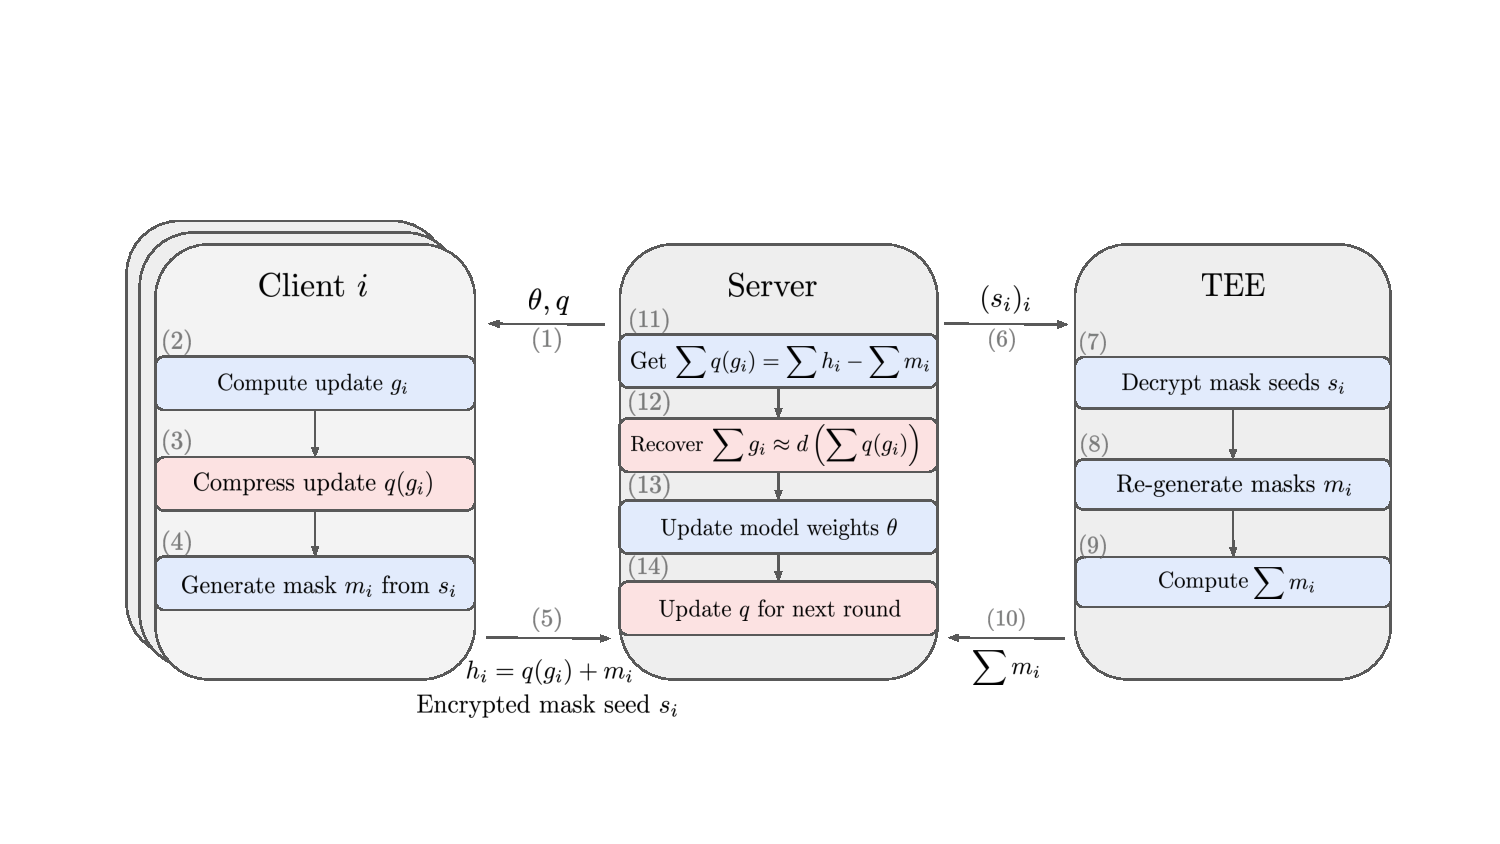
\includegraphics[width=0.8\textwidth]{figs/secagg_summary_new.pdf}
    %\vspace{-5mm}
    \caption{\label{fig:secagg_summary}
    Summary of the proposed approach for one FL round, where we omit the round dependency and \modif{Differential Privacy (DP)} for clarity. Blue boxes denote standard steps and red boxes denote additional steps for uplink compression. Client $i$ computes local model update $g_i$, compresses it with the compression operator $q$, and encrypts it by adding a random mask $m_i$ in the compressed domain, hence reducing the uplink bandwidth (steps 2--4). The server recovers the aggregate in the compressed domain by leveraging any \SecAgg protocol \modif{(steps 7--13, with a TEE-based \SecAgg, see Section~\ref{subsec:secagg})}. Since the decompression operator $d$ is linear, the server can convert the aggregate back to the non-compressed domain, up to compression error (step 12). As with the model weights $\theta$, the compression operator $q$ are also periodically updated and broadcast by the server (step 14). 
    In Section~\ref{sec:method}, we apply the proposed method to scalar quantization and pruning without impacting \SecAgg and propose Secure Indexing, a variant of \SecAgg for extreme uplink compression with product quantization. See Section~\ref{subsec:secagg} for details about \SecAgg and Section~\ref{sec:discussion} for a discussion on~DP.
    }
    \vspace{-3mm}
\end{figure*}



% Our focus in this paper is on 

%Second, scaling cross-device (synchronous) FL to millions of clients with various capabilities and intermittent availability \citep{bonavitz2019federated} suffers from diminishing returns: the wall-clock training time plateaus as the number of clients keeps increasing~\citep{huba2021papaya}. Even though this challenge can be addressed by leveraging the buffered asynchronous aggregation technique proposed by \cite{nguyen2021federated}, compatible with DP and SecAgg, the asynchronous protocol remains bottlenecked by communication latency between the server and the clients.


%Considering the above privacy and scalability goals, we focus on enabling efficient FL communications while keeping a high privacy bar. In addition to the primary objective of speeding up convergence, reducing communication costs brings other significant benefits. Lowering communication requirements addresses selection bias due to undersampling clients with limited connectivity, improving fairness and inclusivity metrics. Better communication efficiency shrinks the carbon footprint of FL, whose fraction attributable to communication can reach 95\%~\citep{qiu2021first}. %Finally, training larger model in FL would be a possibility, when the communication cost is reduced, because local memory or compute requirements can be addressed by modifying the local training loop, for instance with gradient checkpointing \citep{chen2016training}. However, some form of compression would be required to enable efficient communication.


%First, compressing model updates from the client to the server presents several challenges due to compatibility with SecAgg and is an area suitable for further research. 
%Second, upload bandwidth is generally more restricted than download. For instance, according to the most recent FCC report, the ratio of download to upload speeds for DSL/cable providers in the US ranges between 3$\times$ to 20$\times$~\citep{fcc-broadband}. We consider broadband speeds here because devices participate in the FL training while connected to fixed broadband, usually through Wi-Fi~\citep{huba2021papaya}.




% Hence, FL provides the ability to leverage data from massive client populations while ensuring the security and privacy of the client data.
% Go further: compatibility with DP / compression as a mitigation techniques of attacks
% Model and gradient compression intrinsically different.
%  Why not having the secure enclave perform the aggregation?
%!TEX root = ../main.tex
\section{An Overview of DeepEye}
\label{sec:system}

\subsection{System Architecture}

%\add{Rename the layers to be consistent with Introduction.}
We present \sys, an end-to-end framework to prepare data, select visualizations and allow easy-to-use interactions. An overview of \sys is given in Figure~\ref{fig:framwork}, which consists of three layers: {\em (task-driven) data preparation layer}, {\em (smart) data analytics layer}, and {\em user interaction layer}.
%
%\add{!!!!}
%
Data preparation is responsible for crawling daily updated data from different sources, and cleaning them when needed (Section~\ref{subsec:dp}).
%
Data analytics describes the process of both which charts will always be shown (\eg a heat map on a world map showing new cases of every country), and how to automatically recommend visualizations that are ``interesting'' \wrt new incoming data, for visual analytics (Section~\ref{subsec:vs}).
%
Interaction allows a user to explore various and (maybe) new COVID-19 stories in an interactive fashion (Section~\ref{subsec:ie}).


\subsection{Task-driven Data Preparation Layer}
\label{subsec:dp}

%%%%%%%%%%%%%%%%%%%%%%%%%%%%%%%%%%%%
\begin{figure}[t!]
	\centering
	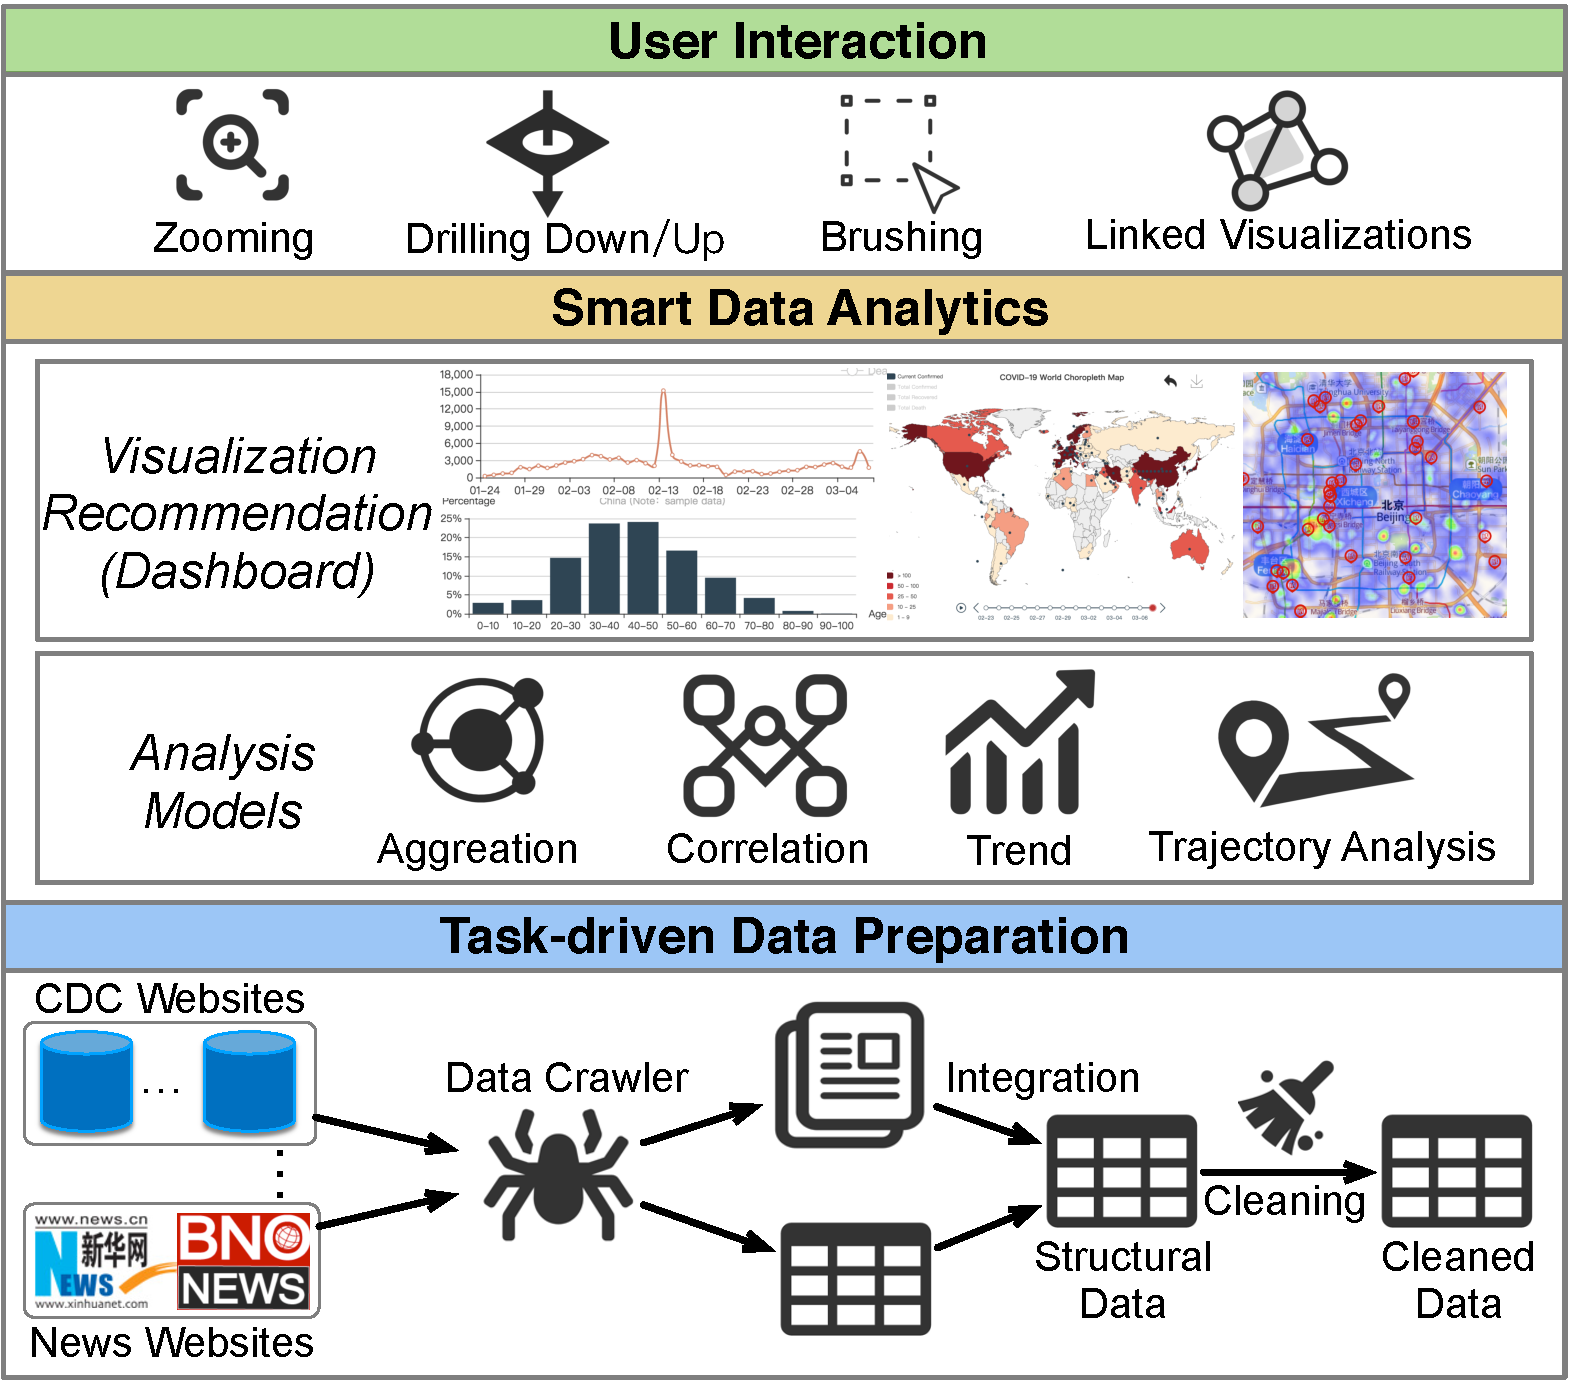
\includegraphics[width=.6\columnwidth]{figs/framework.pdf}
	\caption{System Overview}
	\label{fig:framwork}
\end{figure}
%%%%%%%%%%%%%%%%%%%%%%%%%%%%%%%%%%%%


This layer has a predefined pipeline to prepare data, which will run periodically, with the following three steps.

\stitle{Data Collection.}
We collect data from the following data sources.
(1) We download hourly the official data from the Chinese Center for Disease Control and Prevention (CDC) and other countries' CDCs.
(2) We crawl infected cases' age and gender from authoritative news websites.
(3) We also connect to other data sources like population statistics, temperature data, and so on. 
(4) We are also provided with trajectory data of (potentially) infected persons from China Mobile Limited\footnote{We are collaborating with the company and got mobile phone location data under privacy protection.}. 
%The schema is {\sf S1:}({\sf PhoneID}, {\sf Tag}, {\sf Province}, {\sf City}, {\sf District}, {\sf Address}, { \sf Longitude}, {\sf Latitude}, {\sf Time}).

\stitle{Data Integration.} Next, we need to integrate different types of data into predefined relational tables (\ie global views).
For example, we need to extract report date, location, patients' type, \#-cases from each country's CDC's reports, and  perform schema alignment into  $S1$: ({\em Date, Country, State/Province, City, Total Confirmed, Active Confirmed, Total Deaths, Total Recovered, Death Rate, Recovered Rate, Gender)}, a typical ETL-based data integration process. 


\stitle{Data Cleaning.} After integrating data from multiple sources, there have typical data errors such as duplicates, missing values, synonyms, and so on. 
%\add{Add a sentence to say that we will discuss task-driven data cleaning in Section 3.}
Because data cleaning is known to be tedious and error-prone, we employ our recently proposed technique {\sc VisClean}~\cite{visclean-icde} for visualization-aware data cleaning, which is way cheaper than cleaning the entire dataset. This is doable only after the charts to display have been selected, as discussed below. 
We will depict more details about visualization-aware data cleaning in Section~\ref{sec:dataprep}.

\subsection{Smart Data Analytics Layer}
\label{subsec:vs}
Based on the availability and reliability of data and meta-data, we have successfully conducted the following types of data analytics.

\stitle{Descriptive analytics.} 
We use linked data visualization and visualization recommendation algorithms to effectively show what happened in the past.


\stitle{Diagnostic analytics.} 
We use maps with different layers to test the spatio-temporal properties of COVID-19 data, especially to show the effect of urban (population) density and temperature to the outbreak of COVID-19.


\stitle{Prescriptive analytics.}
Based on the collaboration with companies to get private data, we were able to do some meaningful prescriptive analytics that can recommend actions to decision makers.

%%%%%%%%%%%%%%%%%%%%%%%%%%%%%%%%%%%%
%\begin{figure}[t!]
%	\centering
%	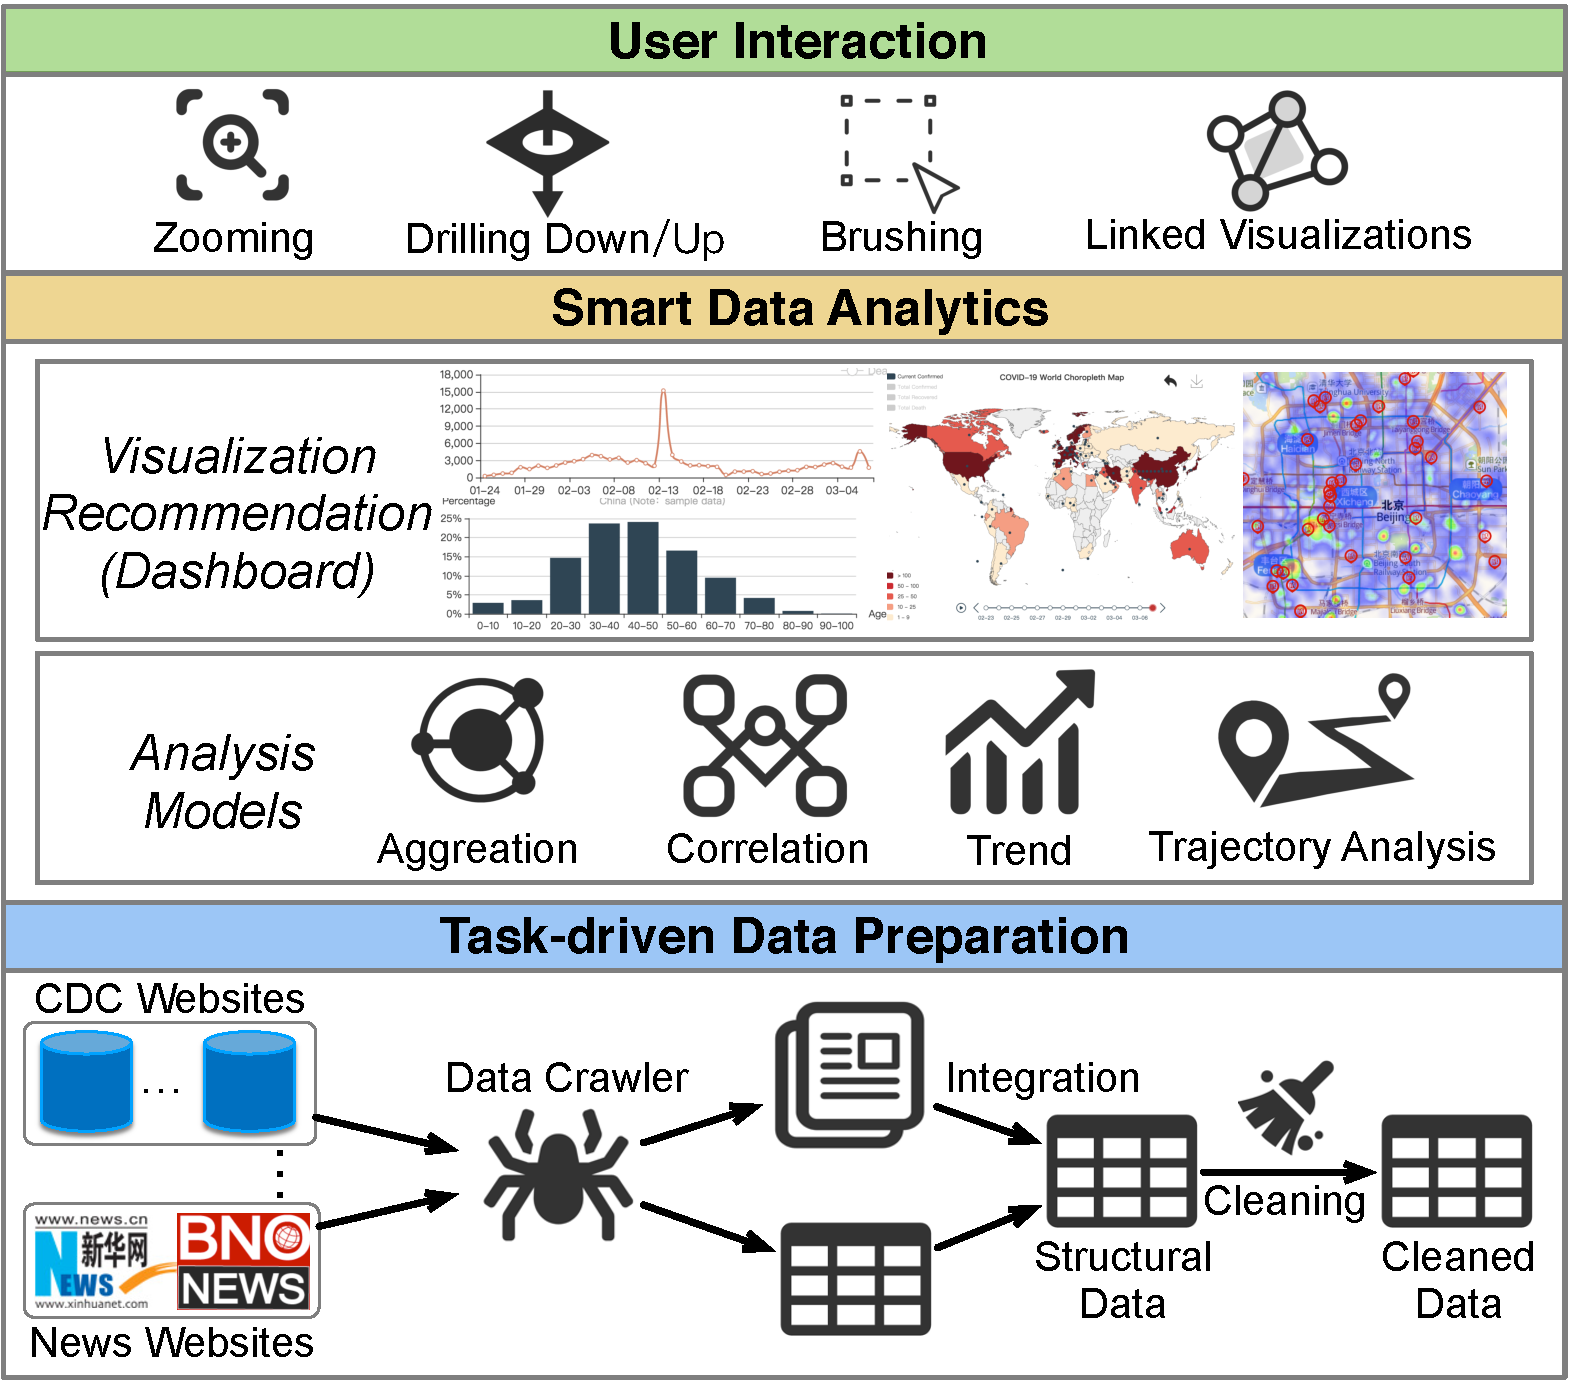
\includegraphics[width=.6\columnwidth]{figs/framework.pdf}
%	%	\vspace{-1.5em}
%	\caption{System Overview}
%	\label{fig:framwork}
%	%	\vspace{-2.5em}
%\end{figure}
%%%%%%%%%%%%%%%%%%%%%%%%%%%%%%%%%%%%





%%%%%%%%%%%%%%%%%%%%%%%%%%%%%%%%%%%%
%\begin{figure*}[t!]
%	\vspace{-1.5em}
%	\centering
%	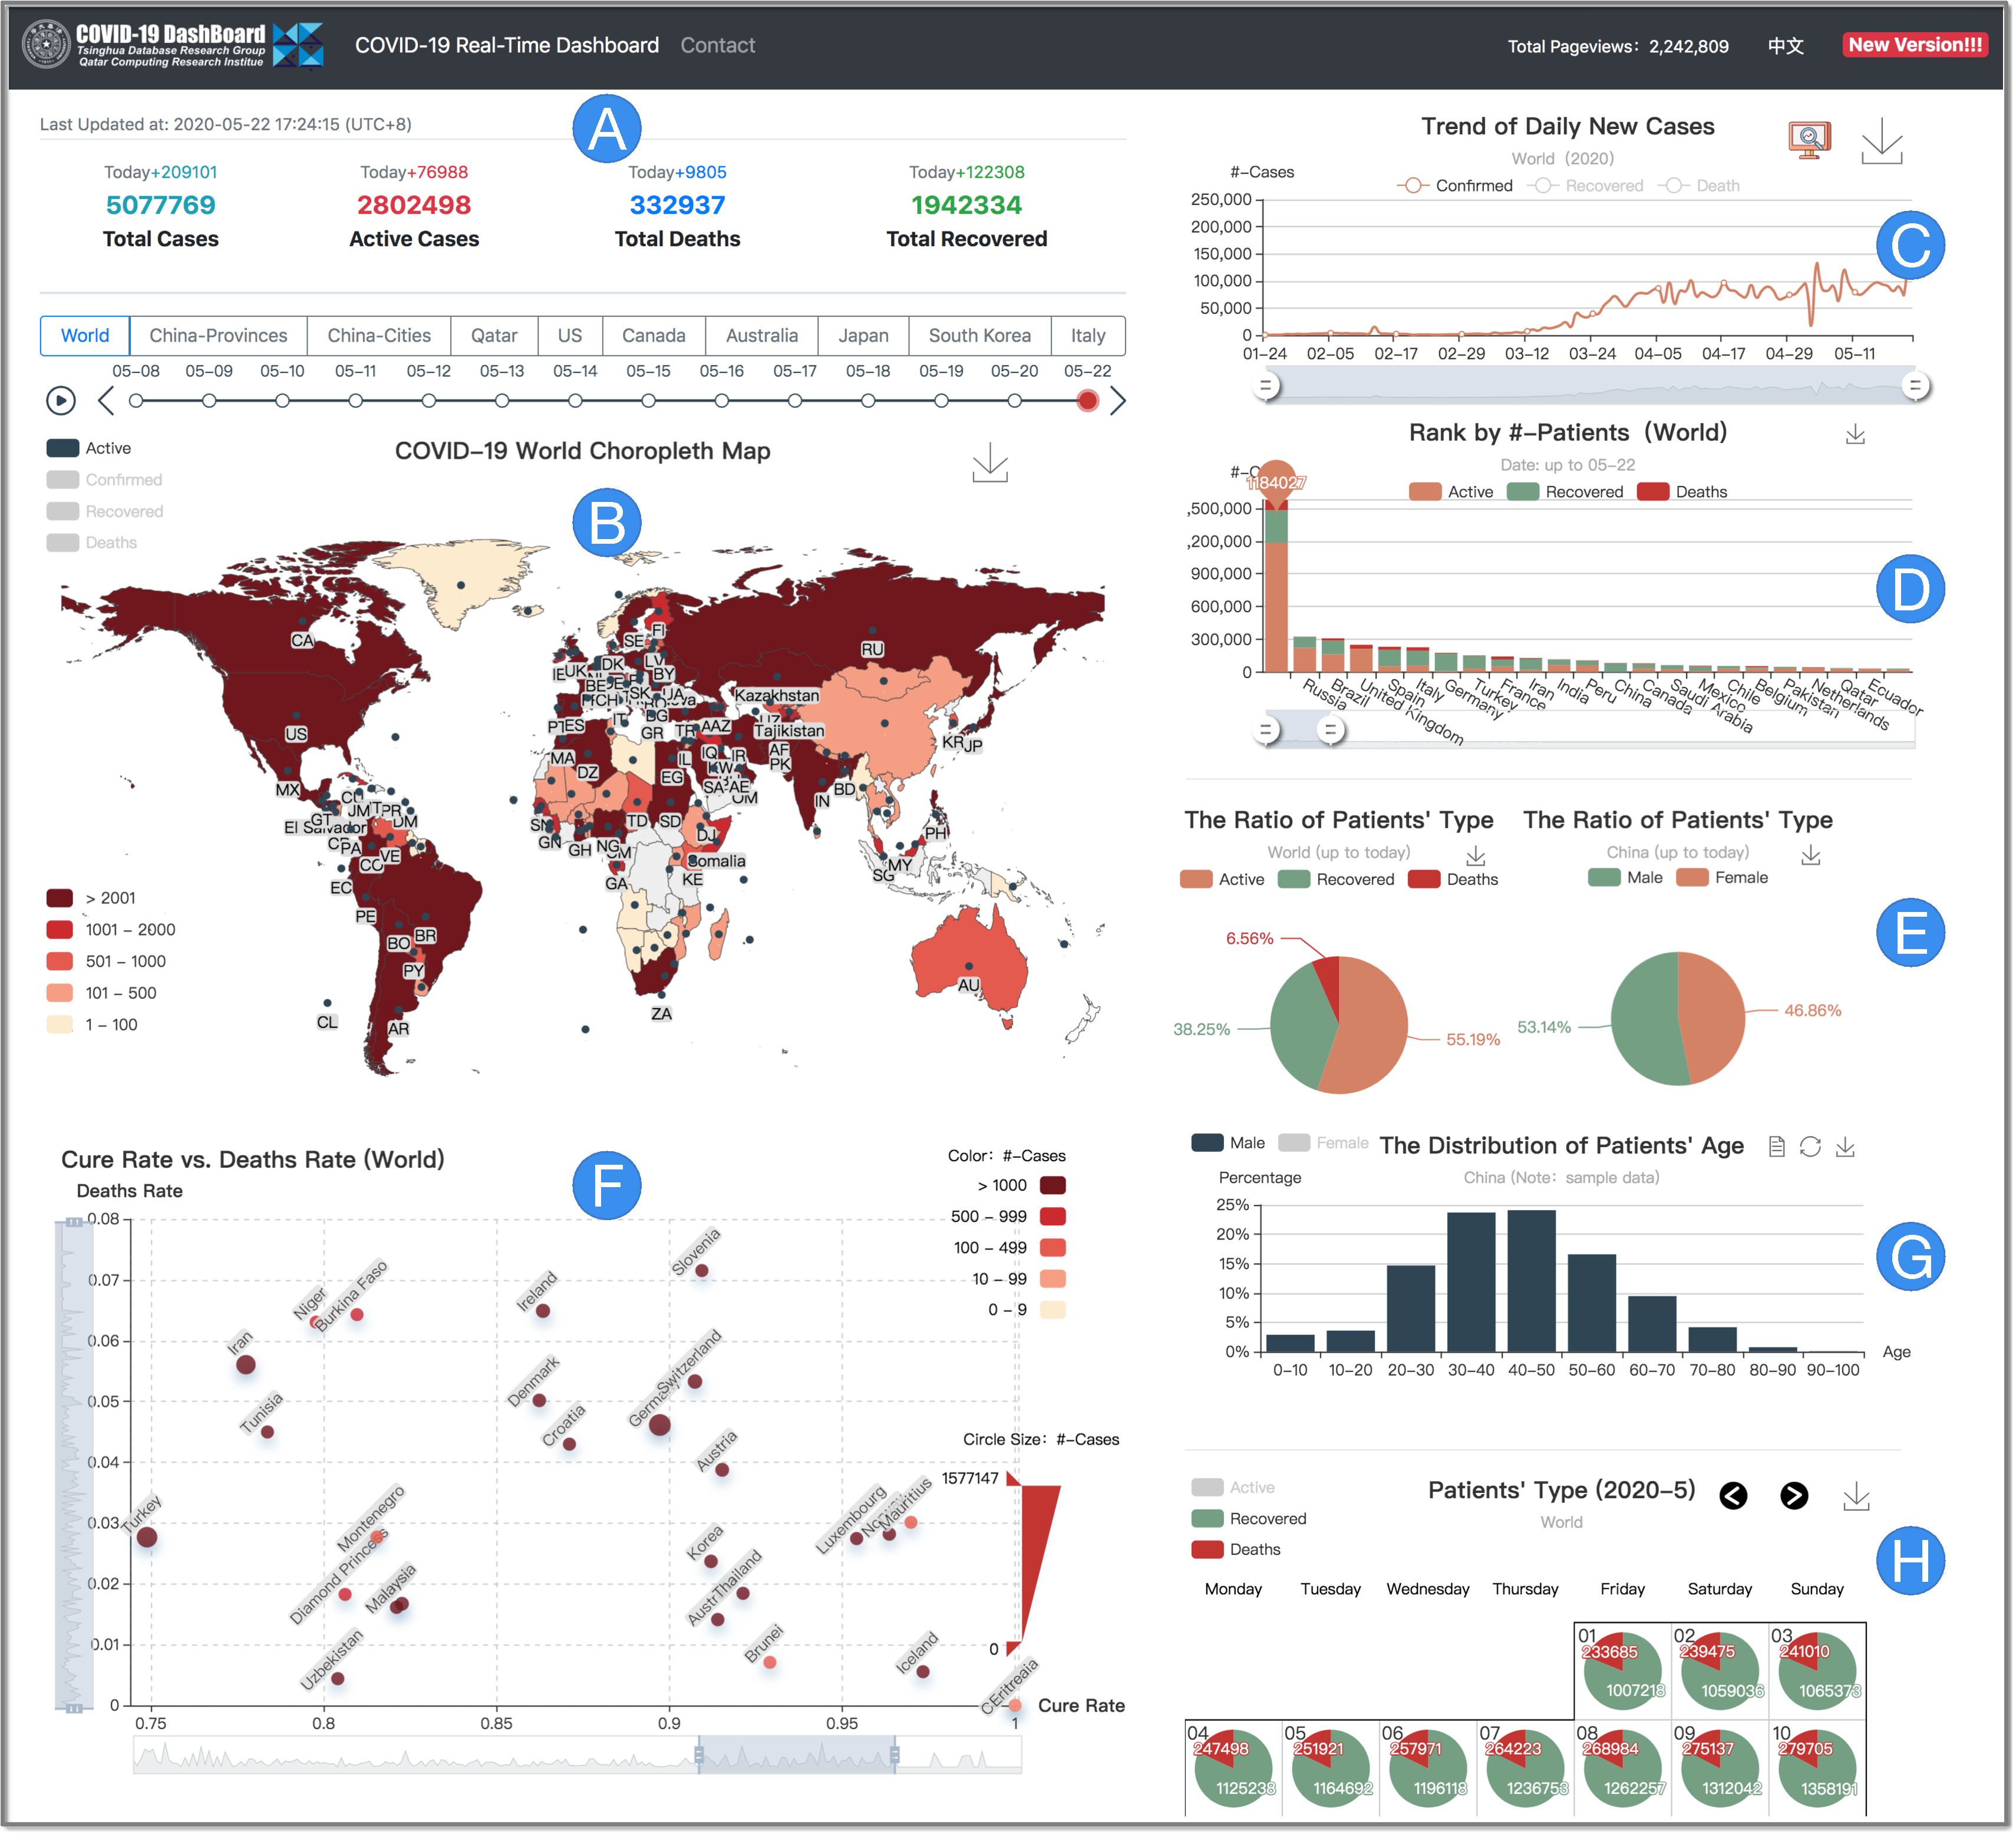
\includegraphics[width=0.9\textwidth]{figs/frontend.pdf}
%	%	\vspace{-1.5em}
%	\caption{Demonstration of \sys-COVID-19 (https://ncov.deepeye.tech/en)}
%	\label{fig:frontend}
%	%	\vspace{-1.5em}
%\end{figure*}
%%%%%%%%%%%%%%%%%%%%%%%%%%%%%%%%%%%%


% \stitle{\sys-COVID-19:}
% We have implemented a \sys instance for COVID-19, which has attracted a broad range of interest from general users, public health authorities, and researchers who want to explore the COVID-19 data and track the outbreak. 
% %


% The base view of \sys-COVID-19 is shown in Figure~\ref{fig:frontend}, which consists of a choropleth map for the total confirmed/recovered/died cases for all countries, line charts for the trend of daily increased cases, calendar charts for visualizing the types of patients, bar charts for distributions of patients' ages, bubble charts for cure rate - death rate, and so on. 
% %
% Besides the basic view page, it also has ad-hoc features, such as tracking infection path and high-risk areas discovery using the trajectory data of infected persons, which will be discussed in Section~\ref{sec:demo}.


% \sys has three layers (see Figure~\ref{fig:framwork}): (1) data preparation, (2) visualization selection, and (3) interaction.
% Next, we will explain each step using the COVID-19 case.


% %%%%%%%%%%%%%%%%%%%%%%%%%%%%%%%%%%%%
% \begin{figure*}[t!]
% 	\centering
% 	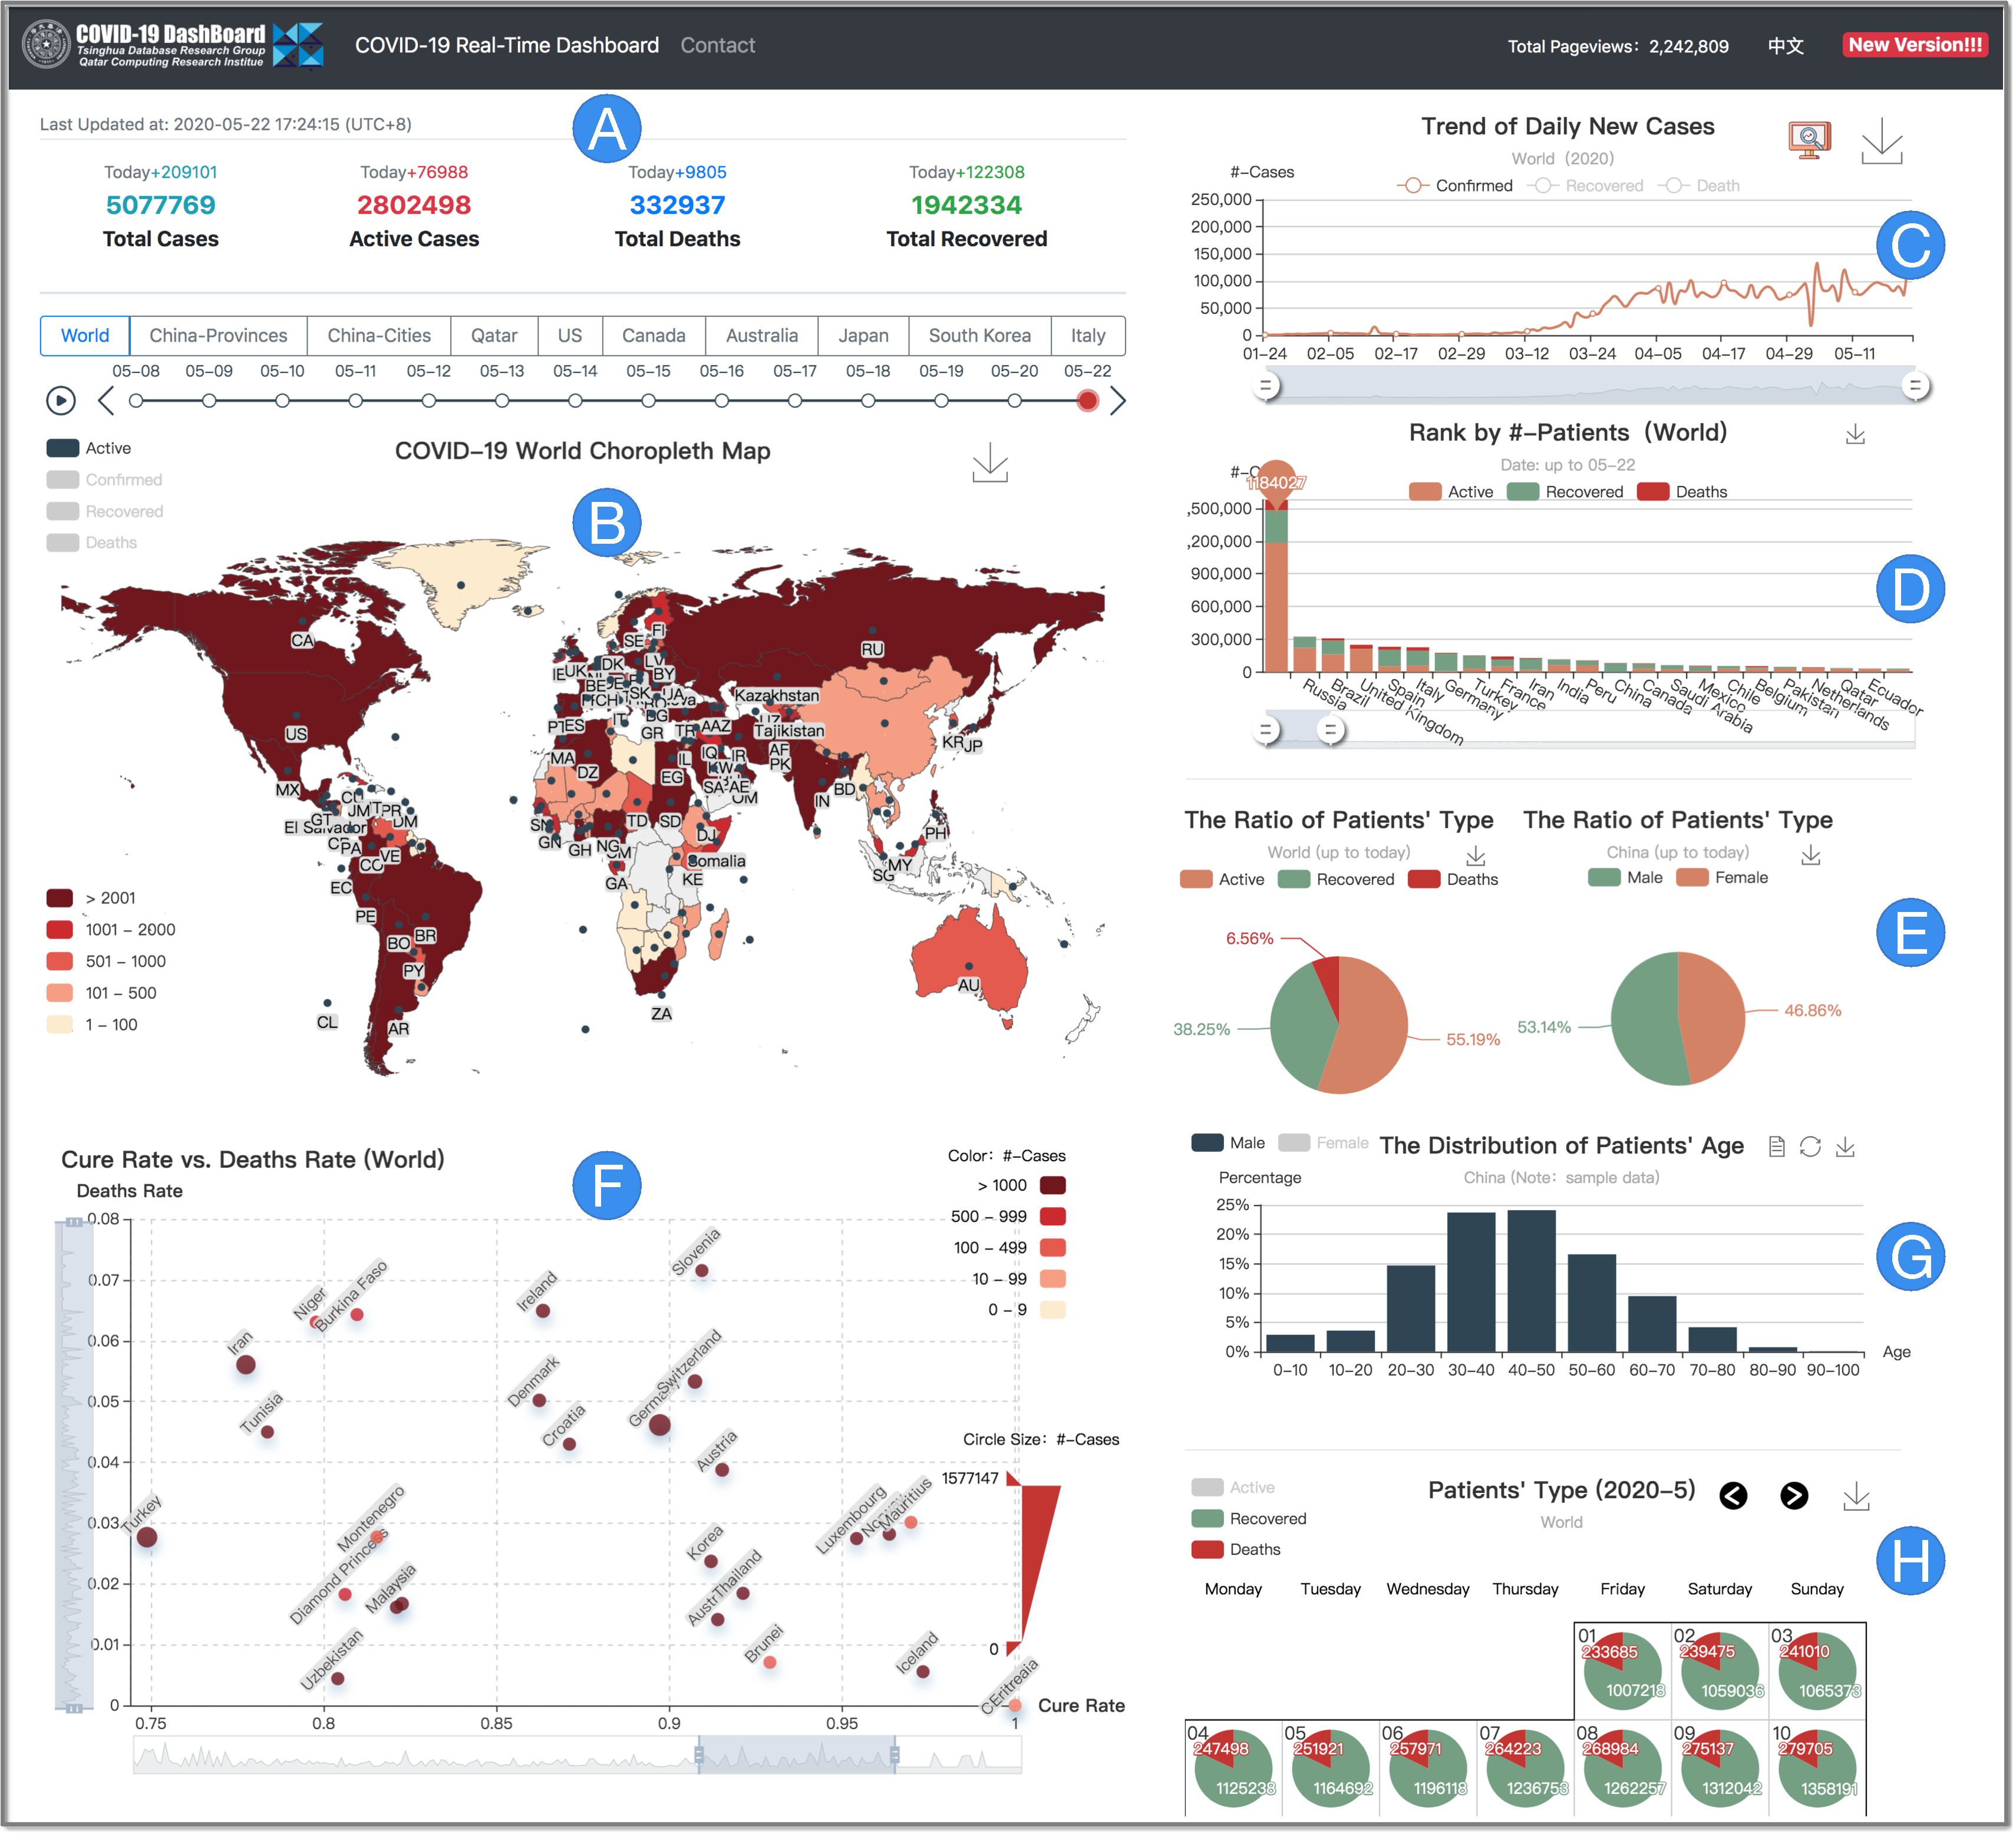
\includegraphics[width=0.9\textwidth]{figs/frontend.pdf}
% 	\caption{Demonstration of \sys-COVID-19 (\lgl{https://ncov.deepeye.tech/en})}
% 	\label{fig:frontend}
% 	\vspace{-.5em}
% \end{figure*}
% %%%%%%%%%%%%%%%%%%%%%%%%%%%%%%%%%%%%






%The data preparation layer, an end-to-end data preparation pipeline, is responsible for collecting, integrating, and cleaning data from multiple data sources. 
%There are some common obstacles in the implementation of this layer. 
%First, we needs to 
%In our application, we collect the reported infected cases from the Chinese Center for Disease Control and Prevention (CDC) and other countries' CDC, and crawler infected cases' age and gender from authoritative news websites, and other data sources like Chinese population statistics.  Moreover, we also gather trajectory data of (potentially) infected persons from China Mobile Limited\footnote{We have collaborated with the company and got mobile phone location data with privacy protection.}. The schema is {\sf S1:}({\sf PhoneID}, {\sf Tag}, {\sf Province}, {\sf City}, {\sf District}, {\sf Address}, { \sf Longitude}, {\sf Latitude}, {\sf Time}).

%Next, we need to integrate different types of data into the relational table.
%For example, we need to extract report date, location, patients' type, \#-cases from each country's CDC's reports, and  perform schema alignment into {\sf S2:}({\sf Date}, {\sf Country}, {\sf State/Province}, {\sf City}, {\sf Total Confirmed}, {\sf Current Confirmed}, {\sf Total Deaths}, {\sf Total Recovered}, {\sf Death Rate}, {\sf Recovered Rate}, {\sf Gender}).

% \stitle{Data Cleaning.} After integrating data from multiple sources, there have typical data errors such as duplicates, missing values, synonyms, and so on. Because data cleaning is known to be tedious and error-prone, we employ our recently proposed technique {\sc VisClean}~\cite{visclean-icde} for visualization-driven data cleaning, which is way cheaper than cleaning the entire dataset. This is doable only after the charts to display have been selected, as discussed below.

%In the above steps, it may introduce some data errors such as duplicates, missing values, and synonyms. 
%Such errors may derive bad visualizations and may misguide users by showing false discoveries. 
%It's necessary to clean the data errors before conduct analysis. However, it is impossible to completely clean a dataset for visualizations (or any other analytical task), simply because data cleaning is prohibitively expensive in terms of the human cost.
%Therefore, we propose to clean those data errors that are relevant to the analysis~\cite{visclean-icde}.

%The system can automatically rerun the pipeline to update data to guarantee its timeliness. 
%Once the pipeline is built, and the data is ready, the next step is to analyze and visualize the data.

% \subsection{Visualization Selection Layer}
% \label{subsec:vs}

% % \add{Paragraph 1: Two types of visualizations are needed. General statistics/trends that can be fixes, and data-driven interesting charts that may be different everyday. So you have Sections 2.2.1 and 2.2.2.}

% Visualization selection generates three categories of charts: {\em linked} common visualizations, {\em ad-hoc} visualizations, and {\em recommended} visualizations.

% \stitle{Linked Common Visualizations.} There are common visualizations for spatial-temporal data exploration, such as a choropleth map (a heat map on a map), line charts to show various trends, bar charts to show the comparison between various groups, scatter charts (or bubble charts) to quantify the relationship between two quantitative variables (\eg death rate vs. cure rate).
% We carefully selected charts (see Figure~\ref{fig:frontend}) that can attract a wide range of interest, and make them ``linked'', \eg when one zoom in from a world level to a country level, all the other charts will be zoomed in, so as to provide a synchronized view from multiple charts.

%%%%%%%%%%%%%%%%%%%%%%%%%%%%%%%%%%%%
\begin{figure}[t!]
	\centering
	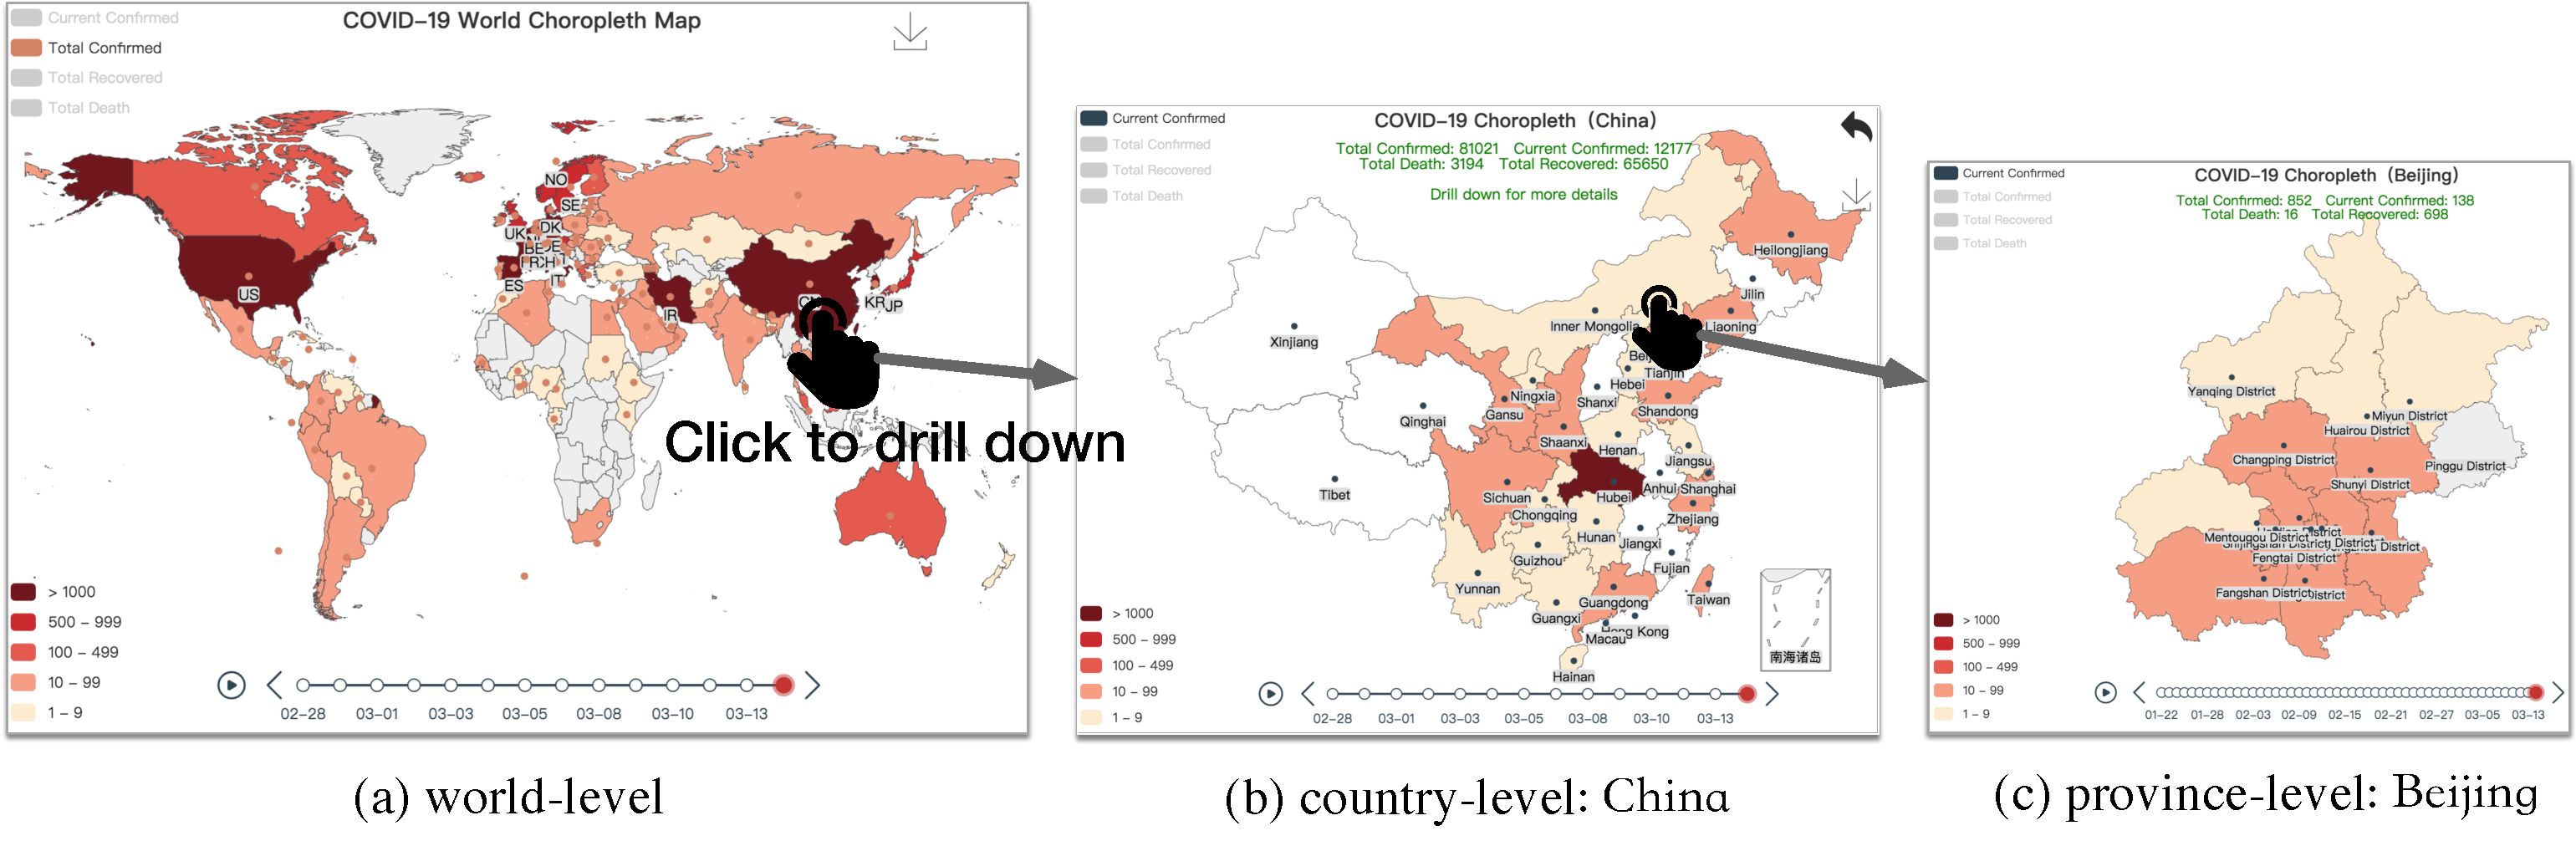
\includegraphics[width=.9\columnwidth]{figs/drill_down_new.pdf}
	\vspace{-1.5em}
	\caption{Drill Down Operation}
	\label{fig:drill_down}
	%	\vspace{-1.5em}
\end{figure}
%%%%%%%%%%%%%%%%%%%%%%%%%%%%%%%%%%%%



\subsection{User Interaction Layer}
\label{subsec:ie}
This is the interface we present to the public.
When a user visits \sys, he/she can further explore visualizations by interactive module for finding more interesting insights. \sys supports popular interactions such as drilling down/up, zooming in/out and linked visualizations, powered by the visualization library ECharts~\cite{DBLP:journals/vi/LiMSSZWZC18}.

Take drill down as an example (see Figure~\ref{fig:drill_down}), when a user clicks a country (\eg China) on the world-level map, the map will drill down into the country-level map for more details.
Note that, \sys provides linked visualizations of the analytical results. That is, when a user performs a drill down operation, other visualizations will also drill down into certain level automatically. In addition, the user can zoom in/out the map by rolling up/down the mouse. 



%It consists of two components, \ie data-dependent visualization design and visualization recommendation. The key points in this layer are (1) what types of visualizations should be designed to interpret the underlying data best; and (2) how to generate such visualizations effectively because there 

% \subsubsection{Data-dependent  Visualization Design}
% For temporal data, there are several common types of visualizations are needed.
% The first type of visualization is line chart, it shows the trend of the temporal data. The second one is bar chart, it shows the distribution or compared information of variables of temporal data, \eg the distribution of the patients' ages.
% Scatter chart (or bubble chart) discovers and quantifies the relationships between two quantitative variables, \eg the death rate v.s. cure rate. 


% \add{Paragraph 1: Maybe you should not call it analysis models, which is not very informative. It should be something like data-dependant chart design or selection, from common ones to special ones, such as infection path or location-based search.}

% It includes a set of data analytical models to process the data for visualization. The analytical models take data as input and output analytical for visualization.
% We implement four types of analysis models in the system. 
% Note that data analysts can plug their analytical model with their domain knowledge into the system, \eg mining the relationships between death rate and medical resources.

% \stitle{Aggregation Analysis.}
% We apply the aggregation analysis to aggregate relational data for visualization. For example, we can use compute the total confirmed cases for each country.

% \stitle{Correlation Analysis.}
% It discovers and quantifies the relationships between two quantitative variables. For example, we can analyze the relationships between \#-cases and recovery (death) rate.

% \stitle{Trend Analysis.}
% For one thing, it records the trend of variables. For another, it can try to predict what will happen in the future.
% In our scenario, we can show the trend of daily increased cases for each country and predict the trend for the coming days. In our system, we use a two-layer neural network $f$ to predict the number of daily confirmed cases in China. The incubation period of the corona virus is 14 days, so we choose the data from the previous 14 days $x=\{c_{-1},c_{-2},...,c_{-14}\}$ as the first input feature and the date of the next day $d$ as the second input feature. We predict the total number of confirmed cases $c = f (x, d)$ the next day. Inspired by the traditional infectious disease model SIR~\cite{kermackcontribution}, we use sigmoid as the activation function in our model $f$.  Gradient descent is used to update the parameters of $f$. By continuously taking the predicted value of the next day as an input, we can continuously predict the confirmed cases in the following days.

% \stitle{Ad-hoc Visualizations}. We also design ad-hoc visualizations to answer specific questions. In terms of COVID-19, besides publicly available datasets, we also have private trajectory data of potentially infected persons. Based on which we have designed two map-based visualizations, one to show infection paths of these patients (see Figure~\ref{fig:infection}), and the other to show the level of risk for each area (see Figure~\ref{fig:heatmap}) and thus suggest the authorities to take different anti-epidemic policies for different areas.

%Besides the above four types of common visualizations, we also need to design some visualizations relevant to analysis scenario.
%Since we also collect the trajectory data of (potential) infected persons.
%Therefore, we use the map to visualize the trajectories. It can benefit us to find such potential infected persons visually, and perform a trajectory similarity search to find a set of similar trajectories to the trajectories of (potential) infected persons. Therefore, we can find a set of high-risk groups. Based on the above analysis, we can further compute the level of risk for each area and thus suggest the authorities take different anti-epidemic policies for different areas.


%\subsubsection{Visualization Recommendation}

% \add{Paragraph 1: Emphasize the requirement of daily news, instead of only daily updates. Why it is hard to have daily news -- a large search space. Naturally, we need some recommendation systems to guide us for doing the job, and we use DeepEye.}

% \stitle{Recommended Visualizations}.
% The above common visualizations are fixed, with data being periodically updated. However, because the data keeps changing, and some interesting stories cannot be captured by predefined common visualizations. Hence, it requires some mechanism to discover these new interesting visualizations, either manually or automatically.
% We leverage our previous work, a visualization recommendation system called {\sc DeepEye}~\cite{deepeyeicde}, to recommend interesting visualizations, such as finding cities in China that share similar trends as Wuhan in terms of death rate. 
% The basic idea of {\sc DeepEye} is to take a table as input, enumerates all possible visualizations of the dataset, select those good visualizations by a supervised classification model, and ranks top-$k$ good visualizations by a learning-to-rank model.

%After we know use what types of visualizations to interpret the data, the next problem is how to process the data for visualization. Not surprisingly, creating good visualizations is not easy in practice, even for the expert. The reason is that it requests the analyst to understand the data both from statistic and semantic perspectives, the right combination of attributes and the right selection of subset. Moreover, the temporal data is usually updated in a certain time interval, and the data feature may also be changed. Thus, the goodness of data-driven visualizations are highly dependent on underlying data.  Therefore, how to select a set of good visualizations after data updating is also a challenge.

%To alleviate the above problem, we propose to use a hybrid method to generate and select good visualizations for the data.  First, we select a set of good visualizations leveraging our previous work, a visualizations recommendation system~\cite{deepeyeicde}. The basic idea of the system is that it takes a relational dataset as input, enumerates all possible visualizations the dataset, select those good visualizations by a classification model, and ranks top-$k$ good visualizations by a learning-to-rank model. Second, we also can manually design good visualizations by incorporating domain knowledge and analysis targets for the dataset. For example, we design a Spatio-temporal choropleth map (\ie choropleth map in Figure~\ref{fig:frontend}) to track the outbreak of COVID-19 around the world visually.  Thus, we select a group of novel visualizations based on the above method and organize those visualizations as a dashboard (See Figure~\ref{fig:frontend}).

% \subsection{Interaction Layer}
% \label{subsec:ie}

% \add{Paragraph 1: You can give some details about the tools you use to implement such a system.}

%Second, what kinds of interactions should we support to enable the visual exploration process more user-friendly.

%\subsection{Interactive Visualization}
%The users also can interact with visualizations to explore the data. 
%
%zoom in, zoom out
%
%drill down, drill up
%
%time line tracking
%
%linking across multiple visualizations

% \stitle{Interaction Types.}

% %%%%%%%%%%%%%%%%%%%%%%%%%%%%%%%%%%%%
% \begin{figure}[t!]
% 	\centering
% 	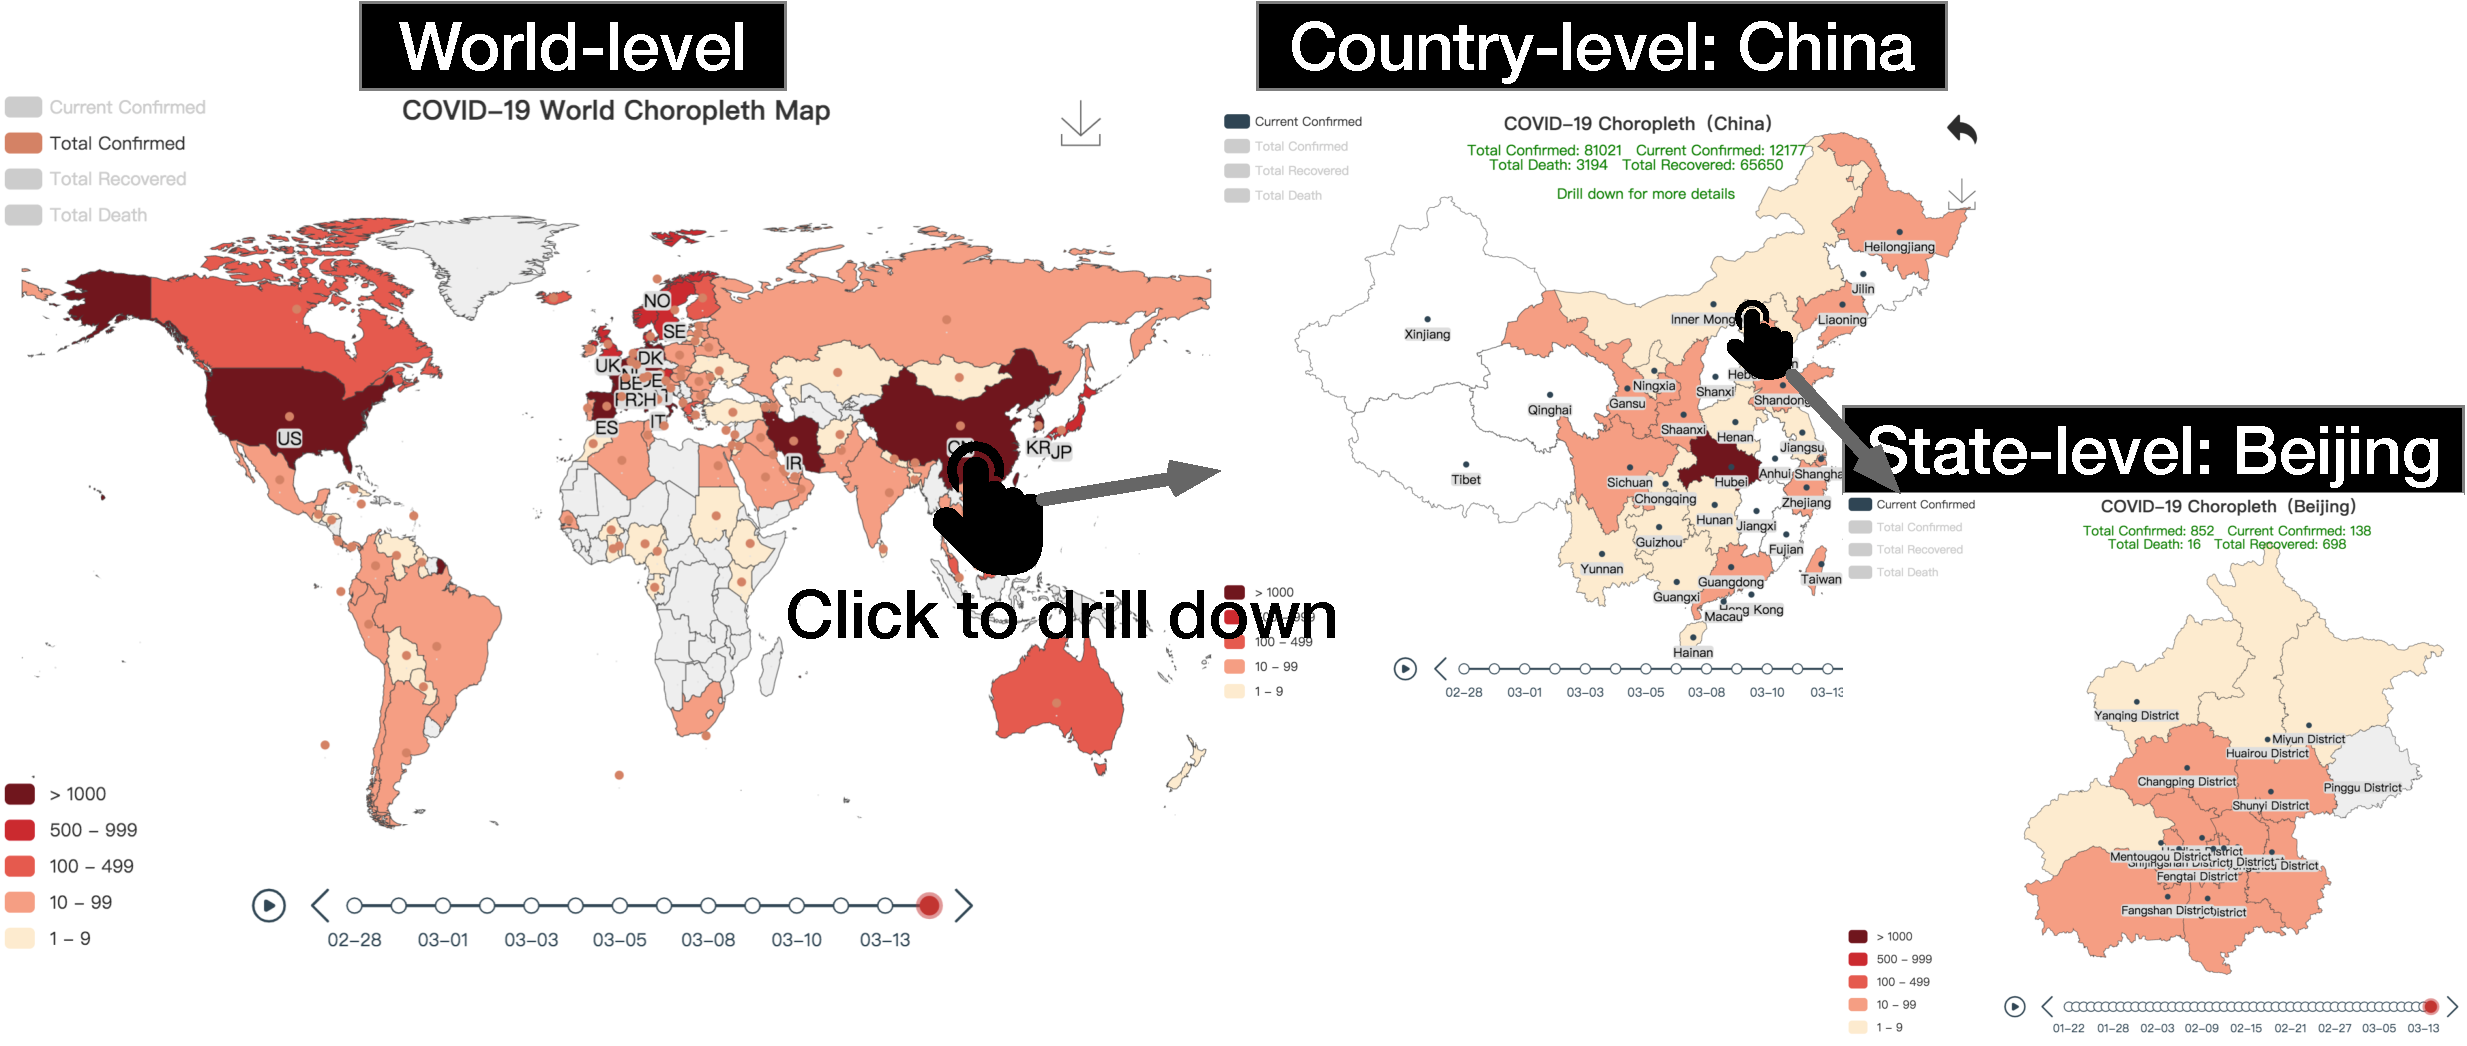
\includegraphics[width=.75\columnwidth]{figs/drill_down.pdf}
% 	\vspace{-1.5em}
% 	\caption{Drill Down Operation}
% 	\label{fig:drill_down}
% %	\vspace{-1.5em}
% \end{figure}
% %%%%%%%%%%%%%%%%%%%%%%%%%%%%%%%%%%%%
% %%%%%%%%%%%%%%%%%%%%%%%%%%%%%%%%%%%%%
% \begin{figure}[t!]
% 	\centering
% 	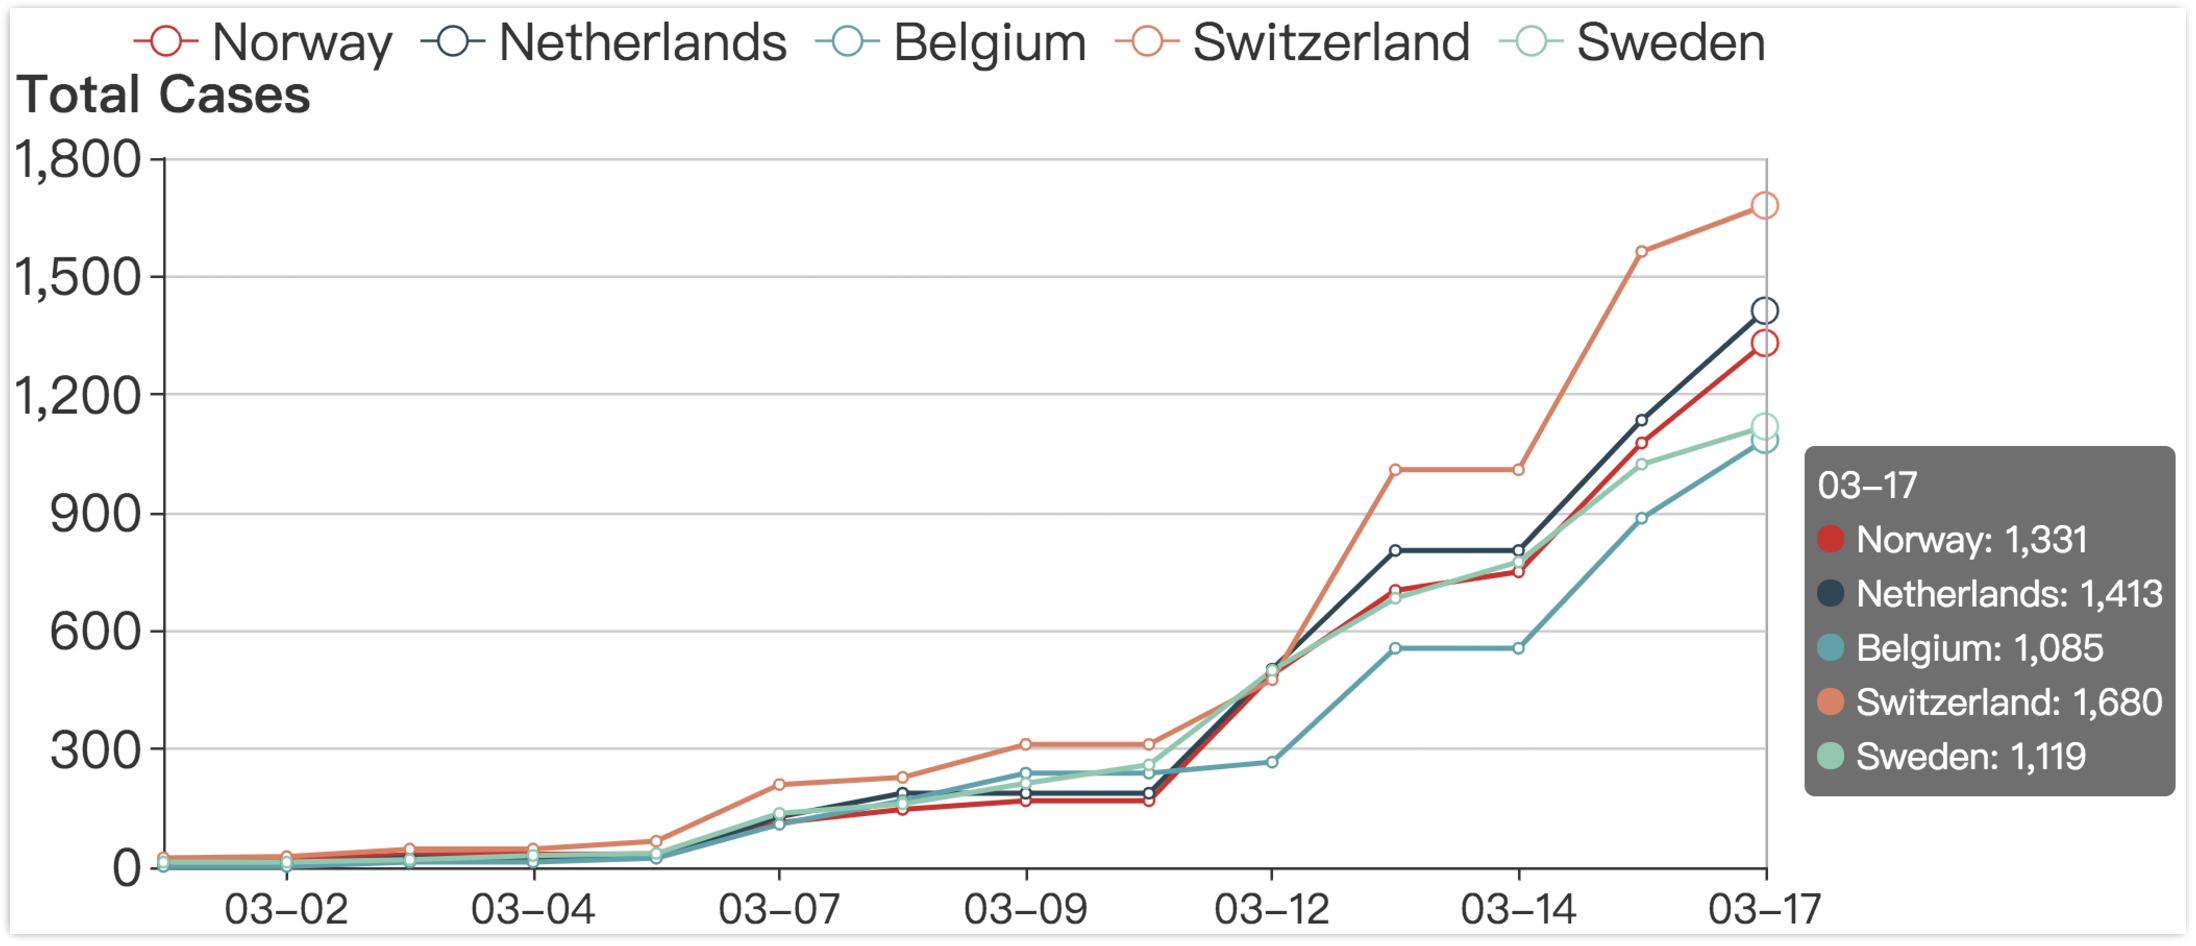
\includegraphics[width=.75\columnwidth]{figs/similarity_trend1.pdf}
% 	\caption{Similar Trend of Confirmed Cases}
% 	\label{fig:similar_trend}
% \end{figure}
% %%%%%%%%%%%%%%%%%%%%%%%%%%%%%%%%%%%%

% \subsection{Interactive Visualization}

% This is the interface we present to the public. 
% When a user visits \sys, he/she can further explore visualizations by interactive module for finding more interesting insights. \sys supports popular interactions such as drilling down/up, zooming in/out and linked visualizations.

% Take drill down as an example (see Figure~\ref{fig:drill_down}), when a user clicks a country (\eg China) on the world-level map, the map will drill down into the country-level map for more details.
% Note that, \sys provides linked visualizations of the analytical results. That is, when a user performs a drill down operations, other visualizations will also drill down into certain level automatically. In addition, the user can zoom in/out the map by rolling up/down the mouse.



% \subsection{How to support reuse and plugin.}
% \label{subsec:disscussion}


%!TEX root = ../main.tex
\section{Human-in-the-loop Machine Learning Pipeline}
\label{sec:pipeline}

As shown in Figure~\ref{fig:framwork}, humans play significant roles in machine learning pipeline. First, given some unstructured data, we have to transform it structured data, in order to construct features for ML. Then for structured data from multiple sources, we should integrate them for enriching data and features to achieve  well-performed ML model. What's more, data is always dirty in the real world. To further improve the performance, we should clean the data, such as repairing records that violate integrity constraint  and  removing outliers and duplicates. Finally, we should annotate the data for building the model. For all above steps in the pipeline, humans can contribute their intelligence to provide high quality training data and improve the ML model. Next, we will introduce what humans can contribute in these steps.



\subsection{Data Extraction}

Extracting structured data from unstructured data is an important problem both in industry and academia, which has been studied broadly from rule-based~\cite{DBLP:conf/acl/LiRC11} systems to ML-based  approaches~\cite{DBLP:conf/wsdm/NakasholeTW11, DBLP:conf/aaai/MitchellCHTBCMG15}. However, these methods either need domain experts to design rules or humans to provide large quantities of labels. Recently, DeepDive~\cite{DBLP:conf/sigmod/Zhang0RCN16} is a representative system in this area, which provides  declarative language  for  non-expert users to extract data.  The execution of DeepDive can be divided into three parts: candidate generation, supervision, statistical inference and learning. Humans mainly contribute in the first part, i.e., candidate generation. In this part, humans write some extraction rules described by declarative languages to retrieve data with attributes or relations, such as  entity B is the wife of A if there exists mention ``and his wife" between A and B in a corpus. The goal of this part is to generate candidates with high recall and low precision. Secondly, the supervision part applies distant supervision rules from knowledge bases or incomplete databases  to provide labels for some of the candidates. The rules do not need to label all candidates from the first part, which are intended to be a low recall and high precision. For the last part, DeepDive constructs a graphical model that represents all of the labeled candidate extractions, trains the model, and then infers a correct probability for each candidate. At the end of this stage, DeepDive applies a threshold to each inferred probability and then derives the extractions to  the output database. In conclusion, Deepdive leverages humans to provide extraction candidates with high recall, uses weak supervision(distance supervision) to label them and finally trains a statistical ML model to fine-tune the labels.
 
 

\subsection{Data Integration}
Given relational tables from multiple sources, in many cases we want to integrate them for extending existing datasets, including features and records. To this end, schema matching~\cite{DBLP:journals/pvldb/ZhangCJC13,DBLP:conf/icde/FanLOTZ14} and entity resolution~\cite{DBLP:crowder, DBLP:transitivity} have to be applied, where the first part is going to align the columns and the second will match records from different tables. Recently, many existing works focused on leveraging human intelligence to achieve these. 

For schema matching, existing works~\cite{DBLP:journals/pvldb/ZhangCJC13} utilize human-machine hybrid approaches to improve the performance. They utilize machine-based  schema matching tools to generate a set of possible matchings, each of which has a probability to be matched. 
They define a correspondence correctness question (CCQ) for humans to answer, which denotes a pair of attributes from two columns, so each matching consists of a set of correspondences. Then the problem is to wisely choose  the correspondences to ask the human to obtain the highest certainty of correct schema matching at the lowest cost. The uncertainty is measured by entropy on top of the probabilities that the tools generate. 
In the correspondence selection, they consider the column correlations, selection efficiency and human quality to match schemes effectively and efficiently. 
Fan et.al~\cite{DBLP:conf/icde/FanLOTZ14} introduce knowledge base together with humans to do schema matching. First, they propose a concept-based approach that maps each column of a  table to the best concept in knowledge bases. This approach overcomes the problem that sometimes values of two columns may be disjoint, even though the columns are related, due to incompleteness in the column values. Second, they develop a hybrid machine-crowdsourcing framework that leverages human intelligence to discern the concepts for ``difficult'' columns. The overall framework assigns the most ``beneficial'' column-to-concept matching tasks to the human under a given budget and utilizes the answers to  infer the best matching. 

After the schemes are aligned, we can integrate different relational tables by the join operation. Traditionally, join is always executed by exact matching between values of attributes from two tables. However, in the real world,  data is  always dirty. For example, ``Apple iPhone 8" and "iPhone 8th" refer to the same entities and should be joined, which cannot be done by a traditional database. Therefore, the human-based join is proposed to address this problem. Wang et.al.~\cite{DBLP:crowder} propose  crowd-based join framework, which generates many candidate pairs, uses similarity based pruning techniques to eliminate dissimilar pairs and ask the crowd to answer the rest  pairs. To further reduce the cost, Wang et.al.~\cite{DBLP:transitivity} leverage the transitivity technique to deduce unknown answers based on current answers from humans. Chai et.al.~\cite{DBLP:journals/vldb/ChaiLLDF18, DBLP:conf/sigmod/ChaiLLDF16} build a partial-order graph based on value similarities of different attributes and utilize the graph to prune pairs that are not necessary to ask. To improve the quality,  Wang et.al.~\cite{DBLP:conf/sigmod/WangXL15} first cluster the entities to be joined  and then leverage humans to refine the clusters. Yalavarthi et.al.~\cite{DBLP:conf/cikm/YalavarthiKK17} select questions judiciously considering the crowd errors.





\subsection{Data Cleaning}

Data is dirty in the real world, which is likely to hurt the ML performance. For example, some values may be out of range (e.g., age is beyond 120 or below 0) or utilize wrong units (e.g., some distances are in meters while other are in kilometers); Some records  refer to the same entity; Integrity constraints (e.d. functional dependencies) are violated among records. Recently, many researchers focused on leveraging human to clean the data. For instance, crowd-based entity resolution~\cite{DBLP:crowder, DBLP:journals/vldb/ChaiLLDF18, DBLP:conf/sigmod/ChaiLLDF16} is applied  to remove duplicates. Chai et.al. ~\cite{DBLP:conf/sigmod/ChaiC00LM20} use human expertises to identify outliers among the data. Specifically, they first utilize machine-based outlier detection algorithms to detect some outlier candidates as well as inlier candidates, and then human is asked to verify these candidates by comparing outlier candidates with inliers.  Chu et.al.~\cite{DBLP:journals/pvldb/ChuOMIP0Y15} clean the  data that violates integrity constraints with the help of knowledge base and humans. They first identify the relationships between columns using knowledge base and then use humans to verify them. Then the discovered relationships can be utilized to detect errors among data, and then these error can be repaired by the knowledge base and humans. 


Recently, a line of interesting data cleaning works focus on cleaning with the  explicit goal of improving the ML results. Wang et al.~\cite{DBLP:conf/sigmod/KrishnanFGWW16} propose a cleaning framework ActiveClean for machine learning tasks. Given a dataset and machine learning model with a convex loss, it selects records that can most improve the performance of the model to clean iteratively. ActiveClean consists of 4 modules, sampler, cleaner, updater and estimator. Sampler is used to select a batch of records to be cleaned. The selection criterion is measured by how much improvement can be made after cleaning a record, i.e., the variation of the gradient, which is estimated by the Estimator. Then the selected records will be checked and repaired by the Cleaner, which can be humans. Next, the Updater updates the gradient based on these verified dirty data. The above four steps are repeated until the budget is used up.
BoostClean~\cite{DBLP:journals/corr/abs-1711-01299} cleans the data where an attribute value is out of range. It takes as input a dataset and a set of functions for detecting errors and repair functions. These functions can be provided by humans. Each pair of detection and repair functions can produce a new model. BoostClean uses statistical boosting to find the best ensemble of pairs that maximize the final performance.
Recently, TARS~\cite{DBLP:journals/pvldb/DolatshahTWP18} was proposed to clean human labels using oracles, which provides two pieces of advice. First, given test data with noisy labels, TARS estimates the performance of the model on  true labels, which is shown to be unbiased and confidence intervals are computed to bound the error. Second, given
training data with noisy labels, TARS determines which examples to be sent to an oracle so as to maximize the expected model improvement of cleaning each noisy label.

\subsection{Iterative Labeling}

After the above steps of data preprocessing,  we can label the data in relational tables for ML tasks. The most  straightforward method is to directly leverage humans to annotate a bunch of data for training. Thus we can adopt the cost control and quality control approaches proposed in Section~\ref{sec:overview} to derive high quality labels with low cost (see ~\cite{DBLP:conf/icde/LiWZF17} for a survey). However, in many cases,  a user does not have enough budget to obtain so many annotations. Therefore, many researchers focused on how to label data iteratively and make the model performance better and better using techniques like active learning or weak supervision.

Mozafari et.al.~\cite{DBLP:journals/pvldb/MozafariSFJM14} use active learning to scale up the human labeling, which can be utilized in two scenarios, the upfront and iterative scenario. In the upfront scenario, the user cares more about the latency than the cost. Therefore, given a budget and an initial model, the algorithm uses a ranker to rank and selects some of the most informative examples to label while the rest are predicted by the model. In the iterative scenario, since the user cares more about the cost, the ranker selects a batch of examples to label, retrains the model and selects again until the budget is used up. There are two strategies (Uncertainty and MinExpError) that the user can choose for ranking.  Leveraging the traditional active learning technique, Uncertainty selects examples that the current model is the most uncertain about.  MinExpError uses a more sophisticated algorithm that considers both  the uncertainty and expected model change. Besides, the work also utilizes the bootstrap theory, which makes the algorithms available to any classifier and also enables parallel processing. Also, active learning techniques in section~\ref{subsec:active_learning} can also be integrated in the framework.

DDLite~\cite{DBLP:conf/sigmod/Ehrenberg0RFR16} leverage human to conduct data programming rather than hand-labeling data, in order to generate large quantities of labels. Given a set of input documents, DDLite aims to produce a set of extracted entities or relation mentions, which consists of four steps. First,  given input documents,  preprocessing like domain-specific tokenizers or parsers  of the raw text has to be performed. Second, DDLite provides a library of general candidate extraction operators, which can be designed by humans. Third, humans develop a set of labeling functions through iterating between labeling some small subsets and analyzing the  performance of  labeling functions.
Lastly,  features are automatically generated for the candidates, and then the model is trained using the labeling functions. The humans then analyze the performance on a test set.

\subsection{Model Training and Inference}

 For different machine learning tasks, there are different techniques that leverage humans' knowledge to train and infer the results,  considering humans' diverse qualities. In this part, we mainly discuss two common ML tasks, classification and clustering, and  show how to leverage human intelligence as well as ML techniques to achieve high quality results.


For classification,  it is expensive to obtain reliable labels to train a model, so multiple humans are required to collect subjective labels.  Raykar et.al.~\cite{raykar2010learning} first proposed a straightforward method that simply utilizes majority voting(MV) to infer labels. However, MV does not consider  features of examples. Therefore, given the human labels and features of examples, they improve the model by considering the true labels as latent variables and utilize the Expectation-Maximization (EM) algorithm to train the model. The parameters include the worker qualities and feature weights. Rodrigues et.al.~\cite{DBLP:conf/aaai/RodriguesP18} also use EM algorithm to jointly learn the parameters of humans and examples. The difference is that they use deep learning to train the model, where a crowd layer is proposed to allow the neural network to learn directly from noisy humans labels in an end-to-end manner. In some cases, acquiring large quantities of labels is expensive, so Atarashi et.al.~\cite{DBLP:conf/aaai/AtarashiOK18} proposed to  learn from a small number of  human labels and unlabeled data   using deep generative model in a semi-supervised way. More specifically,  they leverage the unlabeled data effectively by introducing latent features and a data distribution. Because the data distribution can be complex, they use a deep neural network for the data distribution. 
Classification based on taxonomy is a particular but important task that the labels can consist of a taxonomy. For example, BMW X3 and   BMW X5 belong to  BMW, which belongs to Car. For this scenario, Parameswaran et.al.~\cite{DBLP:journals/pvldb/ParameswaranSGPW11} utilize a human-machine hybrid method to classify the examples on the taxonomy. For example, given a picture of an Audi car, we can ask the humans to label whether it is a BMW car. If not, the children of BMW (BMW X3 and BMW X5) can be pruned. They study how to use the minimum number of questions to get all  the labels.




For clustering, we can also leverage human intelligence to cluster examples that are hard to identify by computers. Following the k-means algorithm,  Heikinheimo et.al.~\cite{DBLP:conf/hcomp/HeikinheimoU13} propose a  human-in-the-loop framework that asks the humans to answer a simple task each time and aggregate all the answers to deduce the final clustering result. Specifically, the simple task is, given a triple with three objects, asking the human to select the one different from the other two objects. First, the algorithm picks a large enough number of triplets from the entire dataset and asks humans to label them. Second, for each example, they compute a penalty score defined as  the number of times the example was chosen to be different. Third, the example having the lowest penalty score is returned. Thus, the centroid example of each cluster is computed and we can obtain the clustering results iteratively. However, this method is expensive because of the large number of triple tasks and cannot generalize when there are new examples. To address this,  Gomes et.al.~\cite{DBLP:conf/nips/GomesWKP11} propose to use a generative  model to infer the clusters. Moreover, it can capture multiple  clustering criteria from diverse viewpoints of humans. For example, given a set of pictures of products, one may want to cluster by brands while another human is likely to cluster by types. Specifically, they divide the entire set into small groups and ask humans to cluster examples in each group. Then considering the humans' quality and labels, \cite{DBLP:conf/nips/GomesWKP11} uses a Bayesian generative model to infer the clustering results.






%!TEX root = ../../../deissue.tex
%!TEX root = ../main.tex
\section{Descriptive Data Analytics of COVID-19}
\label{sec:descriptive}

%\stitle{Linked Visualizations.}



Visualization selection generates three categories of charts: {\em linked} common visualizations, {\em ad-hoc} visualizations, and {\em recommended} visualizations.

\stitle{(General) Linked Visualizations.} There are common visualizations for spatio-temporal data exploration, such as a choropleth map (a heat map based on a map), line charts to show various trends, bar charts to show the comparison between various groups, scatter charts (or bubble charts) to quantify the relationship between two quantitative variables (\eg death rate vs. cure rate).
We carefully selected charts (see Figure~\ref{fig:frontend}) that can attract a wide range of interest, and make them ``linked'', \eg when one zoom in from a world level to a country level, all the other charts will be zoomed in, so as to provide a synchronized view from multiple charts.
%%%%
%%%%
The user can get high-level situations of COVID-19 from Figure~\ref{fig:frontend}.
For example, the user can catch the overall information of the reported cases from Figure~\ref{fig:frontend}(A).
%
The choropleth map in Figure~\ref{fig:frontend}(B) shows the location and number of confirmed cases, deaths and recoveries for all affected countries. It also provides a timeline toolbar for the user to look back upon previous situations, and a user can click the ``$\blacktriangleright$'' button to show an animation.
%
The user can click a country, \eg China, to drill down into the country-level (province-level or city-level) for more details. Since we apply the linked visualization techniques, the rest of the visualizations will also drill down into the country-level.
%
Figure~\ref{fig:frontend}(C), a line chart, illustrates the daily increased cases of the selected location.
%
The stacked bar chart in Figure~\ref{fig:frontend}(D) depicts the number of cases for the selected location.
%
The pie charts in Figure~\ref{fig:frontend}(E) show the proportion of patients' type.
% 
Figure~\ref{fig:frontend}(F), a bubble chart, illustrates the relationships across \#-cases, deaths rate, and cure rate.
%
The bar chart in Figure~\ref{fig:frontend}(G) shows the distribution of patients' age, and the calendar chart in Figure~\ref{fig:frontend}(H) illustrates the proportion of types of reported cases for each day.


%\add{You can copy the description of the demo paper bout A--H to give more details.}



%%%%%%%%%%%%%%%%%%%%%%%%%%%%%%%%%%%%
\begin{figure}[t!]
	\centering
	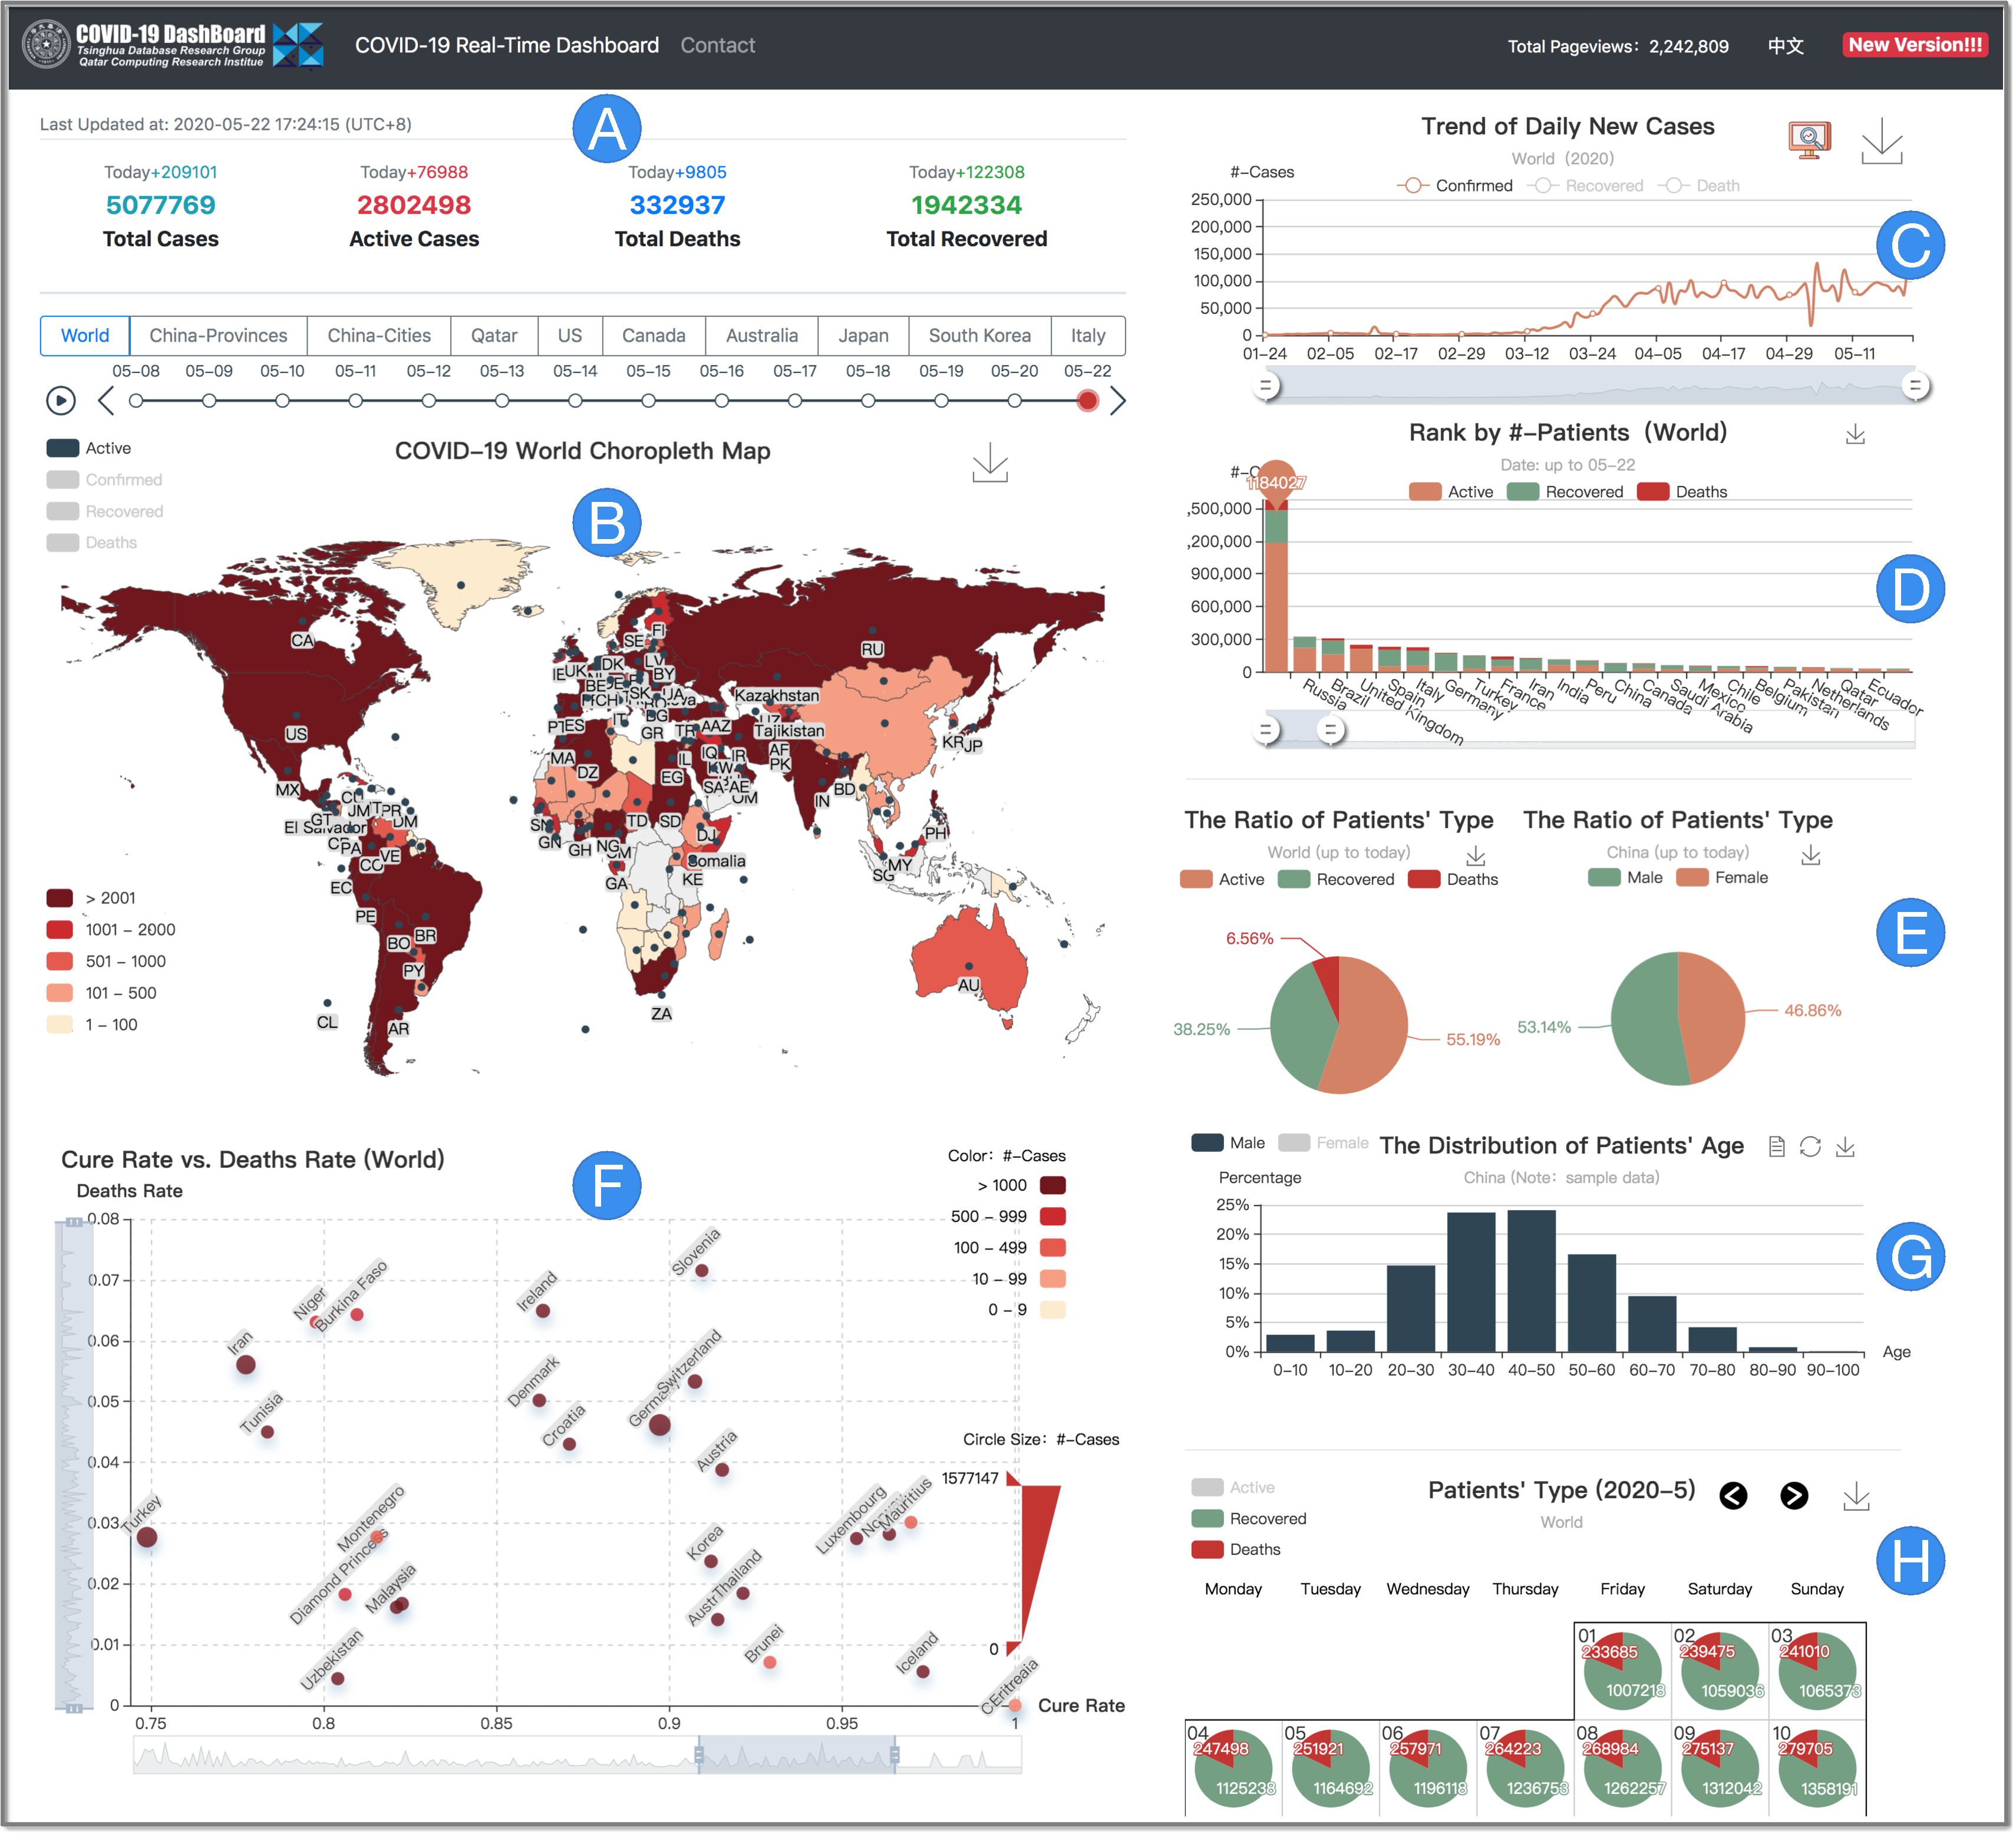
\includegraphics[width=.95\columnwidth]{figs/frontend.pdf}
	\vspace{-1em}
	\caption{The Frontend of \sys (\lgl{https://ncov.deepeye.tech/en})}
	\label{fig:frontend}
	\vspace{-1em}
\end{figure}
%%%%%%%%%%%%%%%%%%%%%%%%%%%%%%%%%%%


%%%%%%%%%%%%%%%%%%%%%%%%%%%%%%%%%%%%

% \begin{figure}[t!]
% 	\begin{subfigure}[b]{0.5\linewidth}
% 		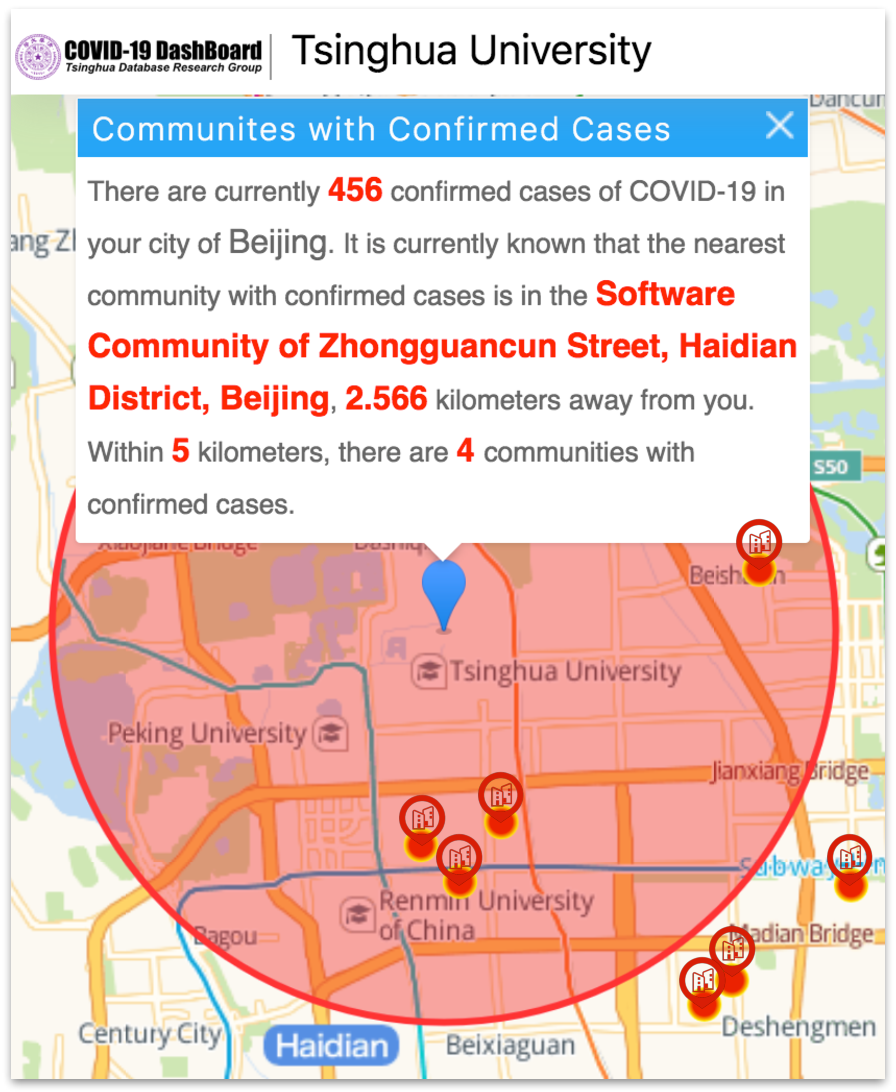
\includegraphics[width=\columnwidth]{{figs/community.pdf}}
% 		\caption{Find Confirmed Cases Around You}
% 		\label{fig:community}		
% 	\end{subfigure}
% 	\begin{subfigure}[b]{0.5\linewidth}
% 		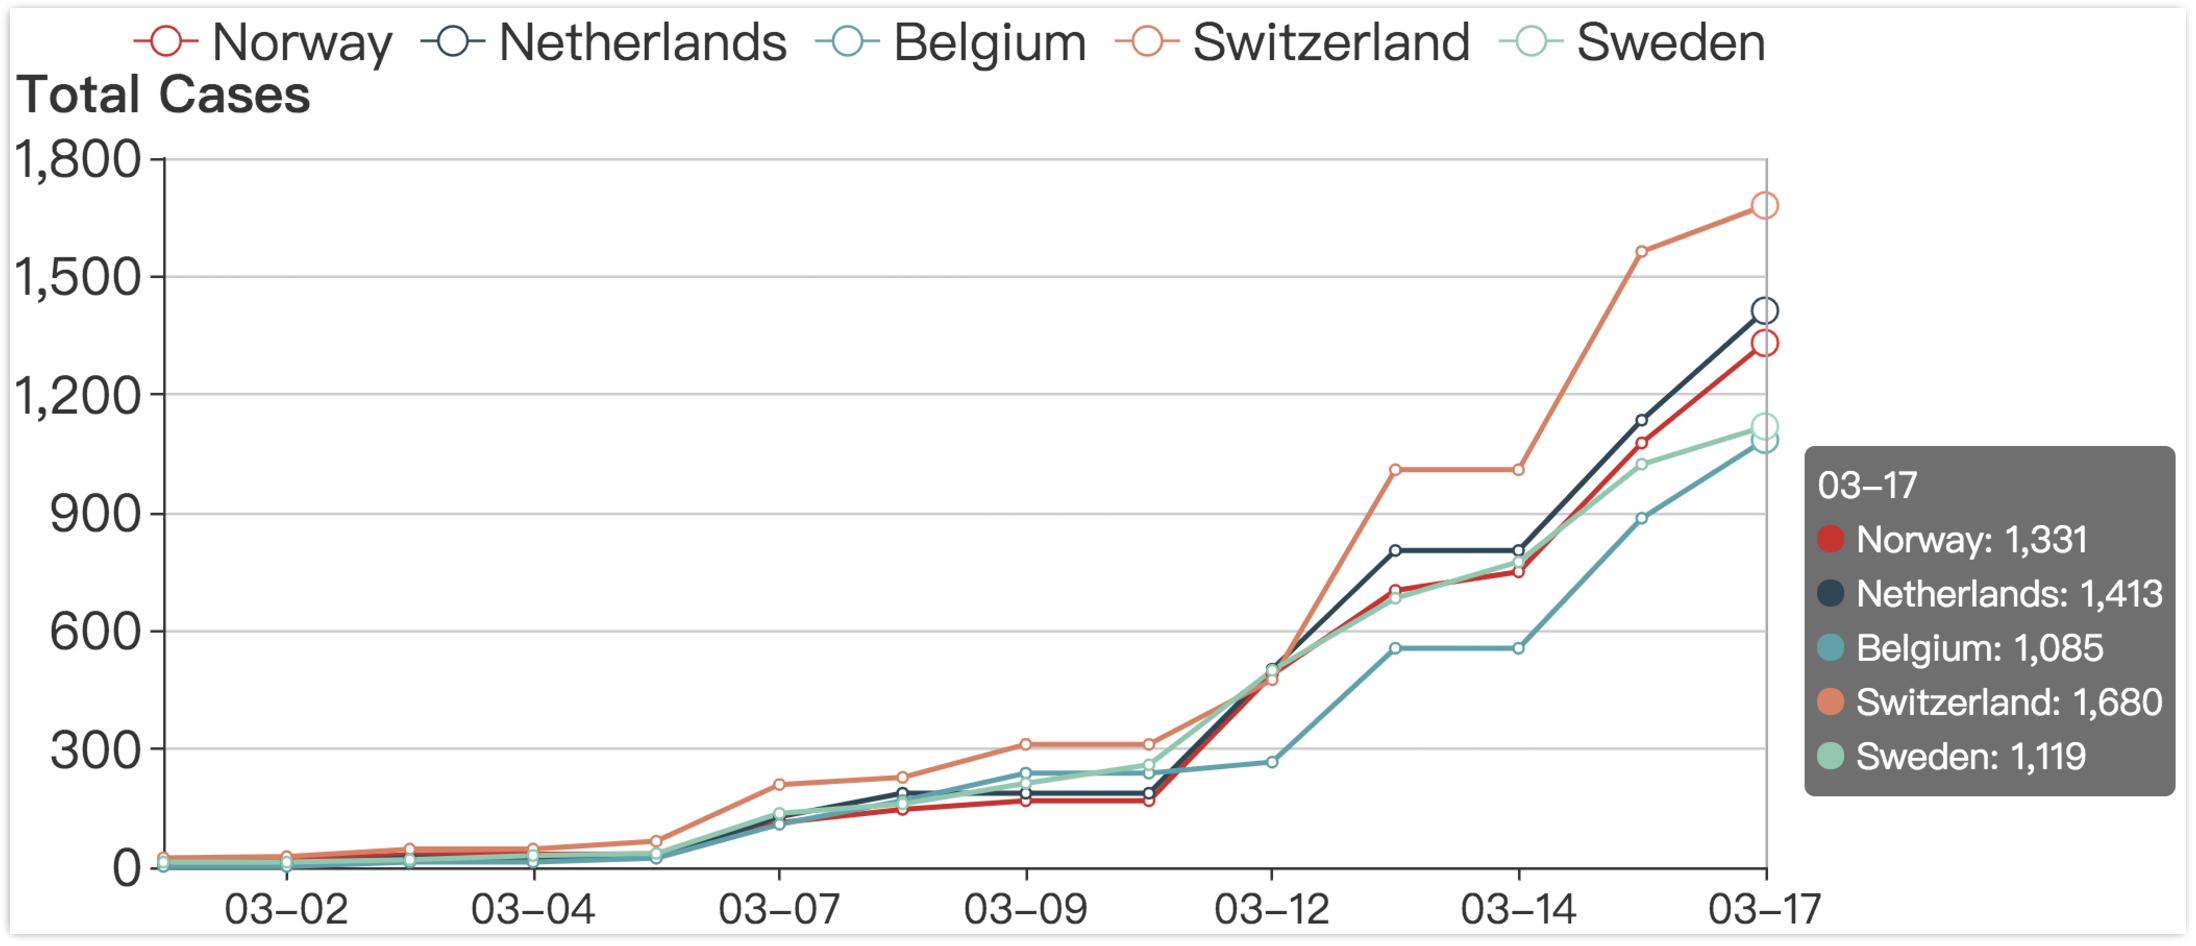
\includegraphics[width=\columnwidth]{figs/similarity_trend1.pdf}
% 		\caption{Similar Trend of Confirmed Cases}
% 		\label{fig:similar_trend}
% 	\end{subfigure}
% \end{figure}


\begin{figure*}[t!]
	\begin{minipage}{\textwidth}
		\centering
		\begin{minipage}{0.4\textwidth}
				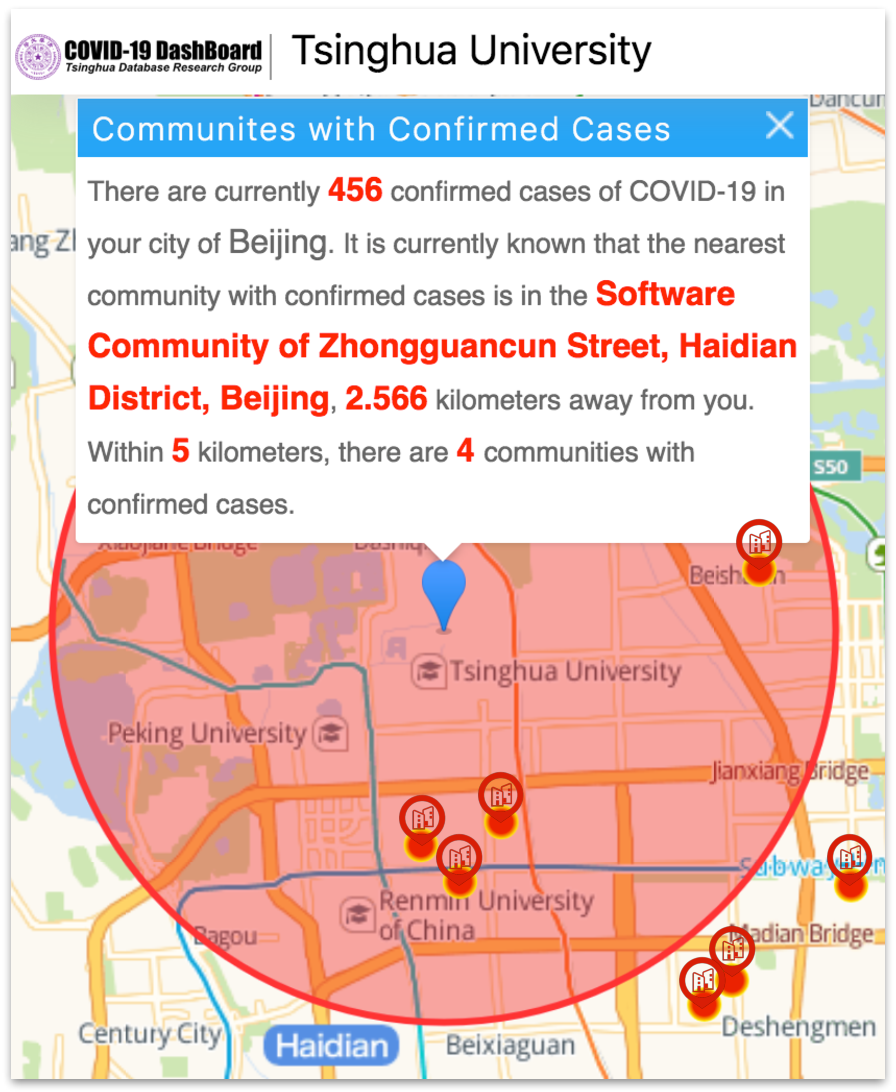
\includegraphics[width=\columnwidth]{{figs/community.pdf}}
				\captionof{figure}{Find Confirmed Cases Around You}
				\label{fig:community}		
		\end{minipage}
		\begin{minipage}{0.59\textwidth}
				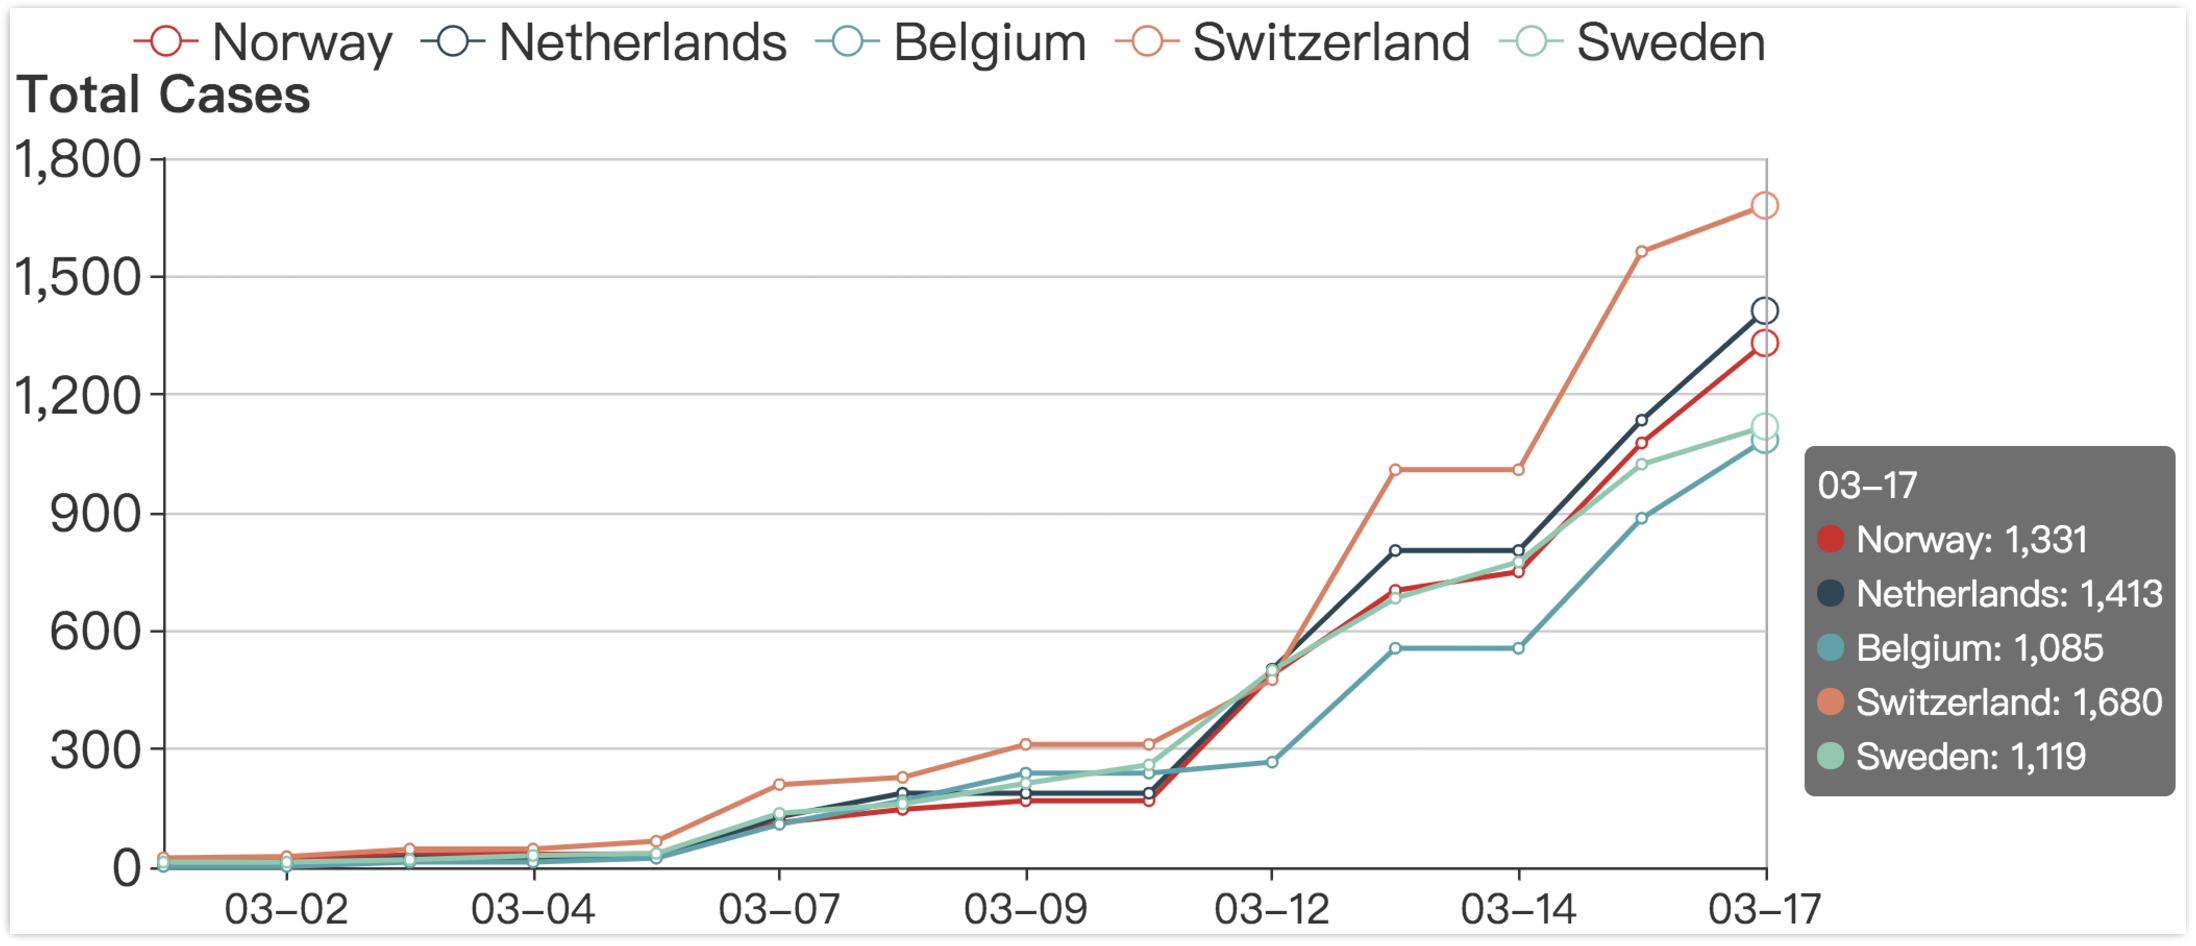
\includegraphics[width=\columnwidth]{figs/similarity_trend1.pdf}
				\captionof{figure}{Similar Trend of Confirmed Cases}
				\label{fig:similar_trend}
		\end{minipage}
	\end{minipage}
\end{figure*}
%%%%%%%%%%%%%%%%%%%%%%%%%%%%%%%%%%%%


%%%%%%%%%%%%%%%%%%%%%%%%%%%%%%%%%%%%
\begin{figure}[t!]
	\centering
	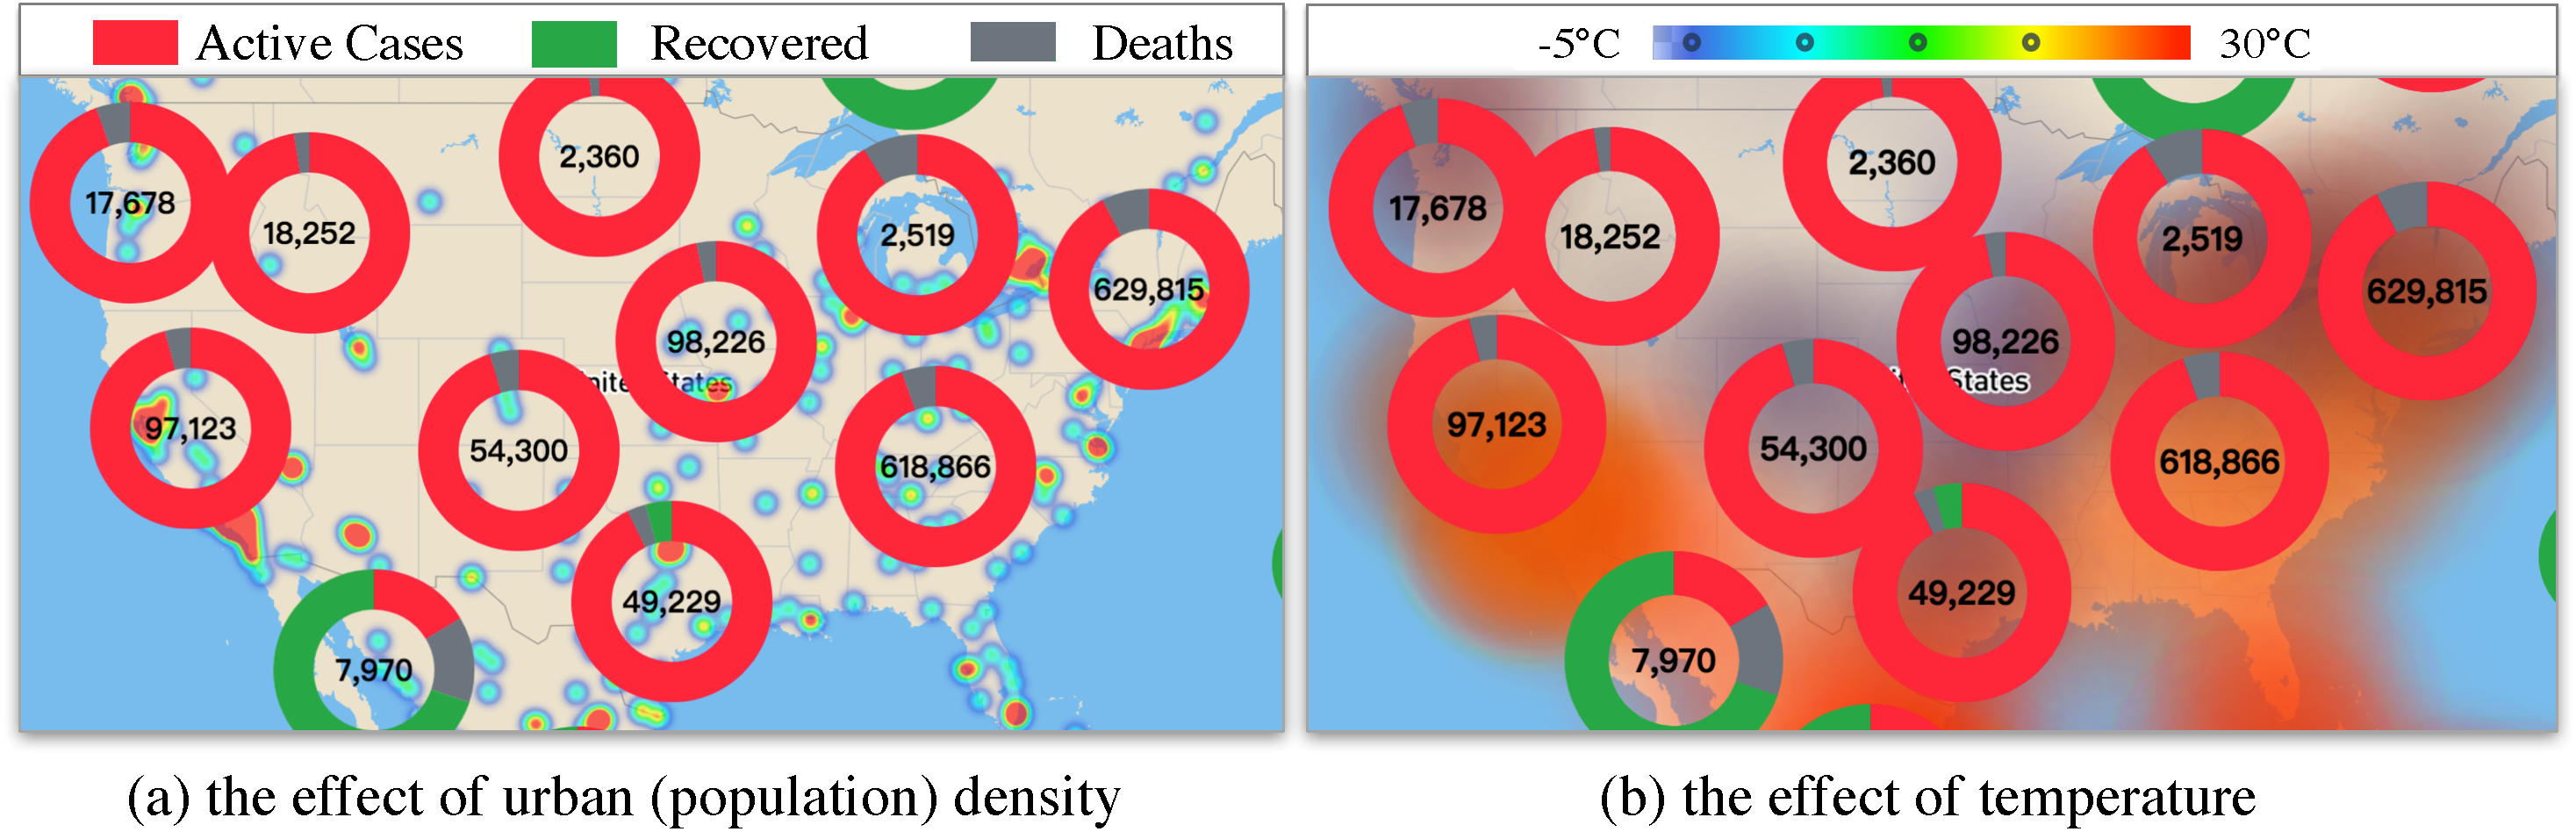
\includegraphics[width=1\columnwidth]{figs/urban_temp.pdf}
	\vspace{-2em}
	\caption{Diagnostic Data Analytics (Case in United States)}
	\label{fig:diagnostic}
	\vspace{-1em}
\end{figure}
%%%%%%%%%%%%%%%%%%%%%%%%%%%%%%%%%%%

\stitle{Location-based Search.}
For the general public, \sys provides the module of finding confirmed cases in nearby neighborhoods. 
Take Figure~\ref{fig:community} for example, users can understand the COVID-19 situations near {\em Tsinghua University, Beijing, China} by a location search box. Note that this module only supports for the Mainland China area currently.

\stitle{Similarity Trends Discovery.}
\sys also supports the similar trend search functionality for finding similar trends. 
%This feature is supported by {\sc DeepEye}~\cite{deepeyeicde} in the back-end.
For example, if the user wants to find those trends of confirmed cases that are similar to {\em Switzerland}, the similarity search functionality will return top-$k$ similar trends about {\em Switzerland}.
The running example is shown in Figure~\ref{fig:similar_trend}. 
Besides line charts,  the similar trend search also supports other charts (\eg bar chart and pie chart).
Thanks to this functionality,  users can perform comparative analysis easier.

\stitle{Automatic News Generation.}
Automatic news generation, in other words, automatically extracting insights from data visualization is promising research and practical direction~\cite{DBLP:journals/vldb/QinLTL20}.
Currently, the user usually interacts with the visualization dashboard to get insights and make decisions. 
For example, the reporter may interact with the dashboard to observe the trend of daily new confirmed cases of each country/state and find a set of similar trends (or find a set of rapidly increasing trends) as news stories.
In this scenario, it heavily relies on the user to manually get insights and write a news release.
One intuitive idea is whether we can derive insights (news stories) from the visualization dashboard automatically. 
%
Roughly speaking, given a set of visualizations $\mathbf{V}$ and a news generation model $\mathbf{M}$, the automatic news generation problem is to output a set of new stories $\mathbf{S}$. 
The key challenge is how to design the news generation model $\mathbf{M}$.
One straightforward approach is predefined a set of expert knowledge rules to mine insights from the visualization dashboard.
%
Such rules can be similar trends discovery, outlier trend detection, trends comparison, and so on.






%!TEX root = ../main.tex
\section{Diagnostic Data Analytics of COVID-19}
\label{sec:diagnostic}
Another purpose of data visualization is to perform hypothesis testing, we show how to design visualizations to test two hypotheses -- urban (population) density \textit{vs.} total confirmed cases, and temperature \textit{vs.} total confirmed cases.

\stitle{Urban (Population) Density.}
One intuitive hypothesis is that whether high population densities catalyze the spread of COVID-19? 
Since we want to know the relationship (correlation) between the population density and the spread of COVID-19, we first visualize the population density in the map named \textit{population density map}, and then we map the confirmed cases on the top of \textit{population density map}. 
As shown in Figure~\ref{fig:diagnostic}(a), it takes United States as an example. It shows that in areas with high population density and without lockdown policy, \eg New York and California, more people are infected with coronavirus.
For example,  New York with a relatively high population density is likely more vulnerable to the spread of the coronavirus. 
This conclusion is reasonable, because the intensive contact greatly increases the probability of coronavirus transmission~\cite{rocklov2020high}.

\stitle{Temperature.}
We also design visualization to show the relationship between the outbreak of COVID-19 and the temperature factor.  Similarly, we first visualize heatmap using temperature data, and then we map the confirmed cases on the top of the heatmap.
As shown in Figure~\ref{fig:diagnostic}(b), it is hard for us to make conclusions like the higher temperature, the more infected cases, or the lower temperature, the less infected cases. 
For example, the average temperature in the central United States is lower than in California, but there are also hundreds of thousands of infected people in the central United States. Comparing Figure~\ref{fig:diagnostic}(a) and Figure~\ref{fig:diagnostic}(b), we can find that under the background of no lockdown, the population density has a stronger correlation with the number of confirmed cases.




%!TEX root = ../main.tex

\section{Concluding Remarks}
\label{conclusion}

There exist many systems for monitoring and analyzing spatio-temporal data, such as a dashboard for visually tracking the outbreak of COVID-19~\cite{dong2020interactive} and a tweet stream sentiment analysis system for US election 2016~\cite{DBLP:conf/kdd/PaulLTYF17}. 
One lesson from the existing systems is  that they are usually designed on a case-by-case basis and built from scratch, which cannot fully leverage the recent techniques for data integration and automatic visualization.

On the one side, \sys-COVID-19 shares many common visualizations as the other popular websites for tracking COVID-19 cases.
On the other side, it differs from the others in 
(1) \sys-COVID-19 is based on a general end-to-end framework \sys, and leverages recent techniques for data preparation (\eg~{\sc VisClean}~\cite{visclean-icde}) and for visualization recommendation (\eg~{\sc DeepEye}~\cite{deepeyeicde});
%
(2) it supports linked visualization for the users to easily zoom in/out multiple visualizations by a single click; and
%
(3) it also obtains some private data that is not publicly available, so it can demonstrate some unique features.
%
%Hopefully we can survive the war of fighting COVID-19 with the minimum cost, and by the time of VLDB 2020, we will have much more to demonstrate.

%\add{Open Challenges: (1) Smart and Effective Data Preparation. (2) Data Sharing Platform. (3) Intelligent Data Analysis (4) Abstract general modules, the system supports reusability}

% \bibliographystyle{abbrv}
% \bibliography{DA}  

\begin{thebibliography}{10}

\bibitem{DBLP:journals/pvldb/AbedjanCDFIOPST16}
Z.~Abedjan, X.~Chu, and et.al.
\newblock Detecting data errors: Where are we and what needs to be done?
\newblock {\em {PVLDB}}, 9(12):993--1004, 2016.

\bibitem{DBLP:conf/cidr/BinnigSKUZZ17}
C.~Binnig, L.~D. Stefani, T.~Kraska, E.~Upfal, E.~Zgraggen, and Z.~Zhao.
\newblock Toward sustainable insights, or why polygamy is bad for you.
\newblock In {\em {CIDR}}.

\bibitem{carcione2020simulation1}
J.~M. Carcione, J.~E. Santos, C.~Bagaini, and J.~Ba.
\newblock A simulation of a covid-19 epidemic based on a deterministic seir
  model.
\newblock {\em arXiv preprint arXiv:2004.03575}, 2020.

\bibitem{dong2020interactive}
E.~Dong, H.~Du, and L.~Gardner.
\newblock An interactive web-based dashboard to track covid-19 in real time.
\newblock {\em The Lancet Infectious Diseases}, 2020.

\bibitem{DBLP:journals/vi/LiMSSZWZC18}
D.~Li, H.~Mei, Y.~Shen, S.~Su, W.~Zhang, J.~Wang, M.~Zu, and W.~Chen.
\newblock Echarts: {A} declarative framework for rapid construction of
  web-based visualization.
\newblock {\em Vis. Informatics}, 2(2):136--146, 2018.

\bibitem{10.14778/3137765.3137833}
G.~Li.
\newblock Human-in-the-loop data integration.
\newblock {\em Proc. VLDB Endow.}, 10(12):2006–2017, Aug. 2017.

\bibitem{visclean-icde}
Y.~Luo, C.~Chai, X.~Qin, N.~Tang, and G.~Li.
\newblock Interactive cleaning for progressive visualization through composite
  questions.
\newblock In {\em ICDE}, 2020.

\bibitem{deepeyeicde}
Y.~Luo, X.~Qin, N.~Tang, and G.~Li.
\newblock {DeepEye: Towards Automatic Data Visualization}.
\newblock In {\em ICDE}, 2018.

\bibitem{DBLP:conf/kdd/PaulLTYF17}
D.~Paul, F.~Li, M.~K. Teja, X.~Yu, and R.~Frost.
\newblock Compass: Spatio temporal sentiment analysis of {US} election what
  twitter says!
\newblock In {\em SIGKDD}, 2017.

\bibitem{DBLP:journals/vldb/QinLTL20}
X.~Qin, Y.~Luo, N.~Tang, and G.~Li.
\newblock Making data visualization more efficient and effective: a survey.
\newblock {\em {VLDB} J.}, 29(1):93--117, 2020.

\bibitem{rocklov2020high}
J.~Rockl{\"o}v and H.~Sj{\"o}din.
\newblock High population densities catalyse the spread of covid-19.
\newblock {\em Journal of travel medicine}, 27(3):taaa038, 2020.

\end{thebibliography}


\end{document}
